% =====================================================================
%  methodology.tex  --  Chapter 4 (single file; the design-basis text of
%  methodology_design_basis_01JUL.tex is MERGED in Section 4.1 -- no
%  \input needed, retire that file from Overleaf).
%
%  REVISION NOTE (this version):
%   1. Formal definitions of quantities shared across chapters now live
%      in the background chapter: F_dH is eq:fdh_definition and the
%      burnup-to-EFPD conversion is eq:efpd. This chapter defines only
%      its own constructs: the optimisation problem, the constraints,
%      the end-of-cycle criterion (eq:eoc, eq:eoc-k), the Monte Carlo
%      estimator (eq:fdh_estimator) and the k-target (eq:ktarget).
%   2. The duplicated \label{sec:meth-core-objective} is removed; the
%      label belongs only to the proxy-validation section.
%   3. The undefined references sec:peaking_statistics,
%      sec:selection_methodology and sec:stopping_rules are replaced by
%      sec:meth-stats and sec:meth-loop.
%   4. Every displayed formula is followed by a term-by-term list with
%      units. Enumerations set as lists. No semicolons, no em dashes.
%
%  Requires: booktabs, amsmath, graphicx.
%  Figures: figs_thesis/th_model_geometry.pdf (generator committed).
% =====================================================================
\providecommand{\openpoint}[1]{\par\noindent\fbox{\parbox{0.97\linewidth}{%
  \textbf{Open point:} #1}}\par}

\chapter{Methodology}
\label{ch:methodology}

This chapter is ordered along the calculation chain, and each part
answers one question:

\begin{enumerate}
  \item \textbf{What is modelled?} The design basis, the reactor model
        and the soluble boron of the coolant.

  \item \textbf{What is asked of the model?} The optimisation problem,
        its objectives and constraints, the structure of the campaigns
        and the design space and formulation of Campaigns 8 and 9.

  \item \textbf{Which derived quantities does the problem need?} The
        leakage-corrected reactivity target, the radial enrichment
        zoning, the burnup limits and the MTC boron limit set by
        the moderator temperature coefficient.

  \item \textbf{How is a design evaluated and the next batch
        chosen?} The transport fidelity and seeding, and the
        surrogate-assisted loop that drives the search.

  \item \textbf{How is the method checked?} The validation of the
        peaking proxy and the validation of the optimisation framework.

  \item \textbf{When may the active batches of a solve be scored?}
        The source-convergence diagnostic, which decides whether the
        fission source of a transport solve was stationary before its
        active batches began.

  \item \textbf{How is a result reproduced?} The computing
        environments, the seed policy and the archived checkpoints.
\end{enumerate}

The definitions shared with the other chapters are not repeated here.
The radial peaking factor and the burnup-to-cycle-length conversion are
defined in Chapter~\ref{ch:background}, and the results of every
campaign are reported in Chapter~\ref{ch:results}.

\section{Design basis and technological conservatism}
\label{sec:design-basis}

The reference small modular reactor is conceived under a deliberate
constraint of \emph{technological conservatism}, which sets two criteria
for the design basis.

\begin{enumerate}
  \item \textbf{Domestic industrial base:} the fuel technology of the
        core is restricted to what is already qualified and in series
        production in Brazil.

  \item \textbf{Western standard PWR practice:} every choice the
        domestic base leaves open is taken from the most widely
        fabricated and best-benchmarked technology in service, which
        for the lattice is the $17\times17$ Westinghouse-type assembly
        of the NuScale-like reference
        specification~\cite{nuscale_htp2_2017,nuscale_like_core_2024}.
        That specification is the published open description of a small
        modular PWR with a $17\times17$ lattice,
        and this work takes from it the geometry, the material
        compositions and the operating conditions that an OpenMC model
        requires. It is a source of inputs in this chapter, and the
        quantitative comparison against it is made in
        Chapter~\ref{ch:results}.
\end{enumerate}

To meet the mission objective, namely a long refuelling interval under
low-enriched uranium (LEU), the first criterion is relaxed on one
point. The enrichment is bounded by the LEU enrichment limit of \SI{19.75}{wt\%} of
Equation~\eqref{eq:leu-box} rather than by the 2 to \SI{5}{wt\%} of
current INB production~\cite{inb_resende}. Every other element of the
design is held inside the two criteria, and three of them follow
directly from those criteria:

\begin{enumerate}
  \item The fuel form is the one in national production: UO$_2$
        ceramic pellets in Zircaloy-4 cladding, fabricated by INB at
        Resende for Angra~1, a Westinghouse plant, and Angra~2, a
        Siemens
        plant~\cite{inb_montagem_ec,eletronuclear_angra1,eletronuclear_angra2}.

  \item The lattice is the $17\times17$ Westinghouse-type assembly,
        under the second criterion. The Angra units are $16\times16$,
        the geometry of an earlier plant generation, while the
        $17\times17$ is the most widely fabricated commercial geometry
        in service today. Its adoption is therefore an incremental
        industrialisation step for the same qualified fuel fabrication
        process, and it carries a validated basis for benchmarking this
        model against the open
        literature~\cite{nuscale_htp2_2017,nuscale_like_core_2024}.

  \item The excess reactivity is held down by gadolinia burnable
        absorbers, the burnable poison of the Angra~2
        fuel~\cite{angra2_gd_2018}. The gadolinia weight fraction and
        the number of poisoned pins are design variables of the
        search.
\end{enumerate}

The result of the work is therefore a set of core designs that this
industrial base can build and that the control system can hold.

\section{Reactor model}
\label{sec:reactor-model}

Two terms recur throughout this chapter. The evaluator is the code
that builds the OpenMC models of one candidate design, runs its
transport and depletion calculations and returns its objectives and
constraints. The archive is the database in which every evaluated
design is stored with its inputs and its results, and it is the record
from which Chapter~\ref{ch:results} is computed.

The model is built in OpenMC~0.15.3~\cite{romano_openmc_2015} with
ENDF/B-VII.1 data, from one parametric design dictionary driving three
fidelities: pin cell, $17\times17$ assembly, and the 32-assembly core.
Figure~\ref{fig:model-geometry} defines the geometry. Panel~(a) marks
the two enrichment zones, the 24 guide tubes and the central instrument
tube. The poisoned-pin patterns are not depicted there, since they are
given in Figure~\ref{fig:gd-ladder}. The ranges of the six design
variables of
Campaigns 5 to 7 are tabulated beneath the panels, where $p$ and
$t_\mathrm{refl}$ appear coupled by $g_\mathrm{geom}$. The numerical
basis is concentrated in Tables~\ref{tab:model-geometry}
and~\ref{tab:model-operating}.

\begin{figure}[htbp]
  \centering
  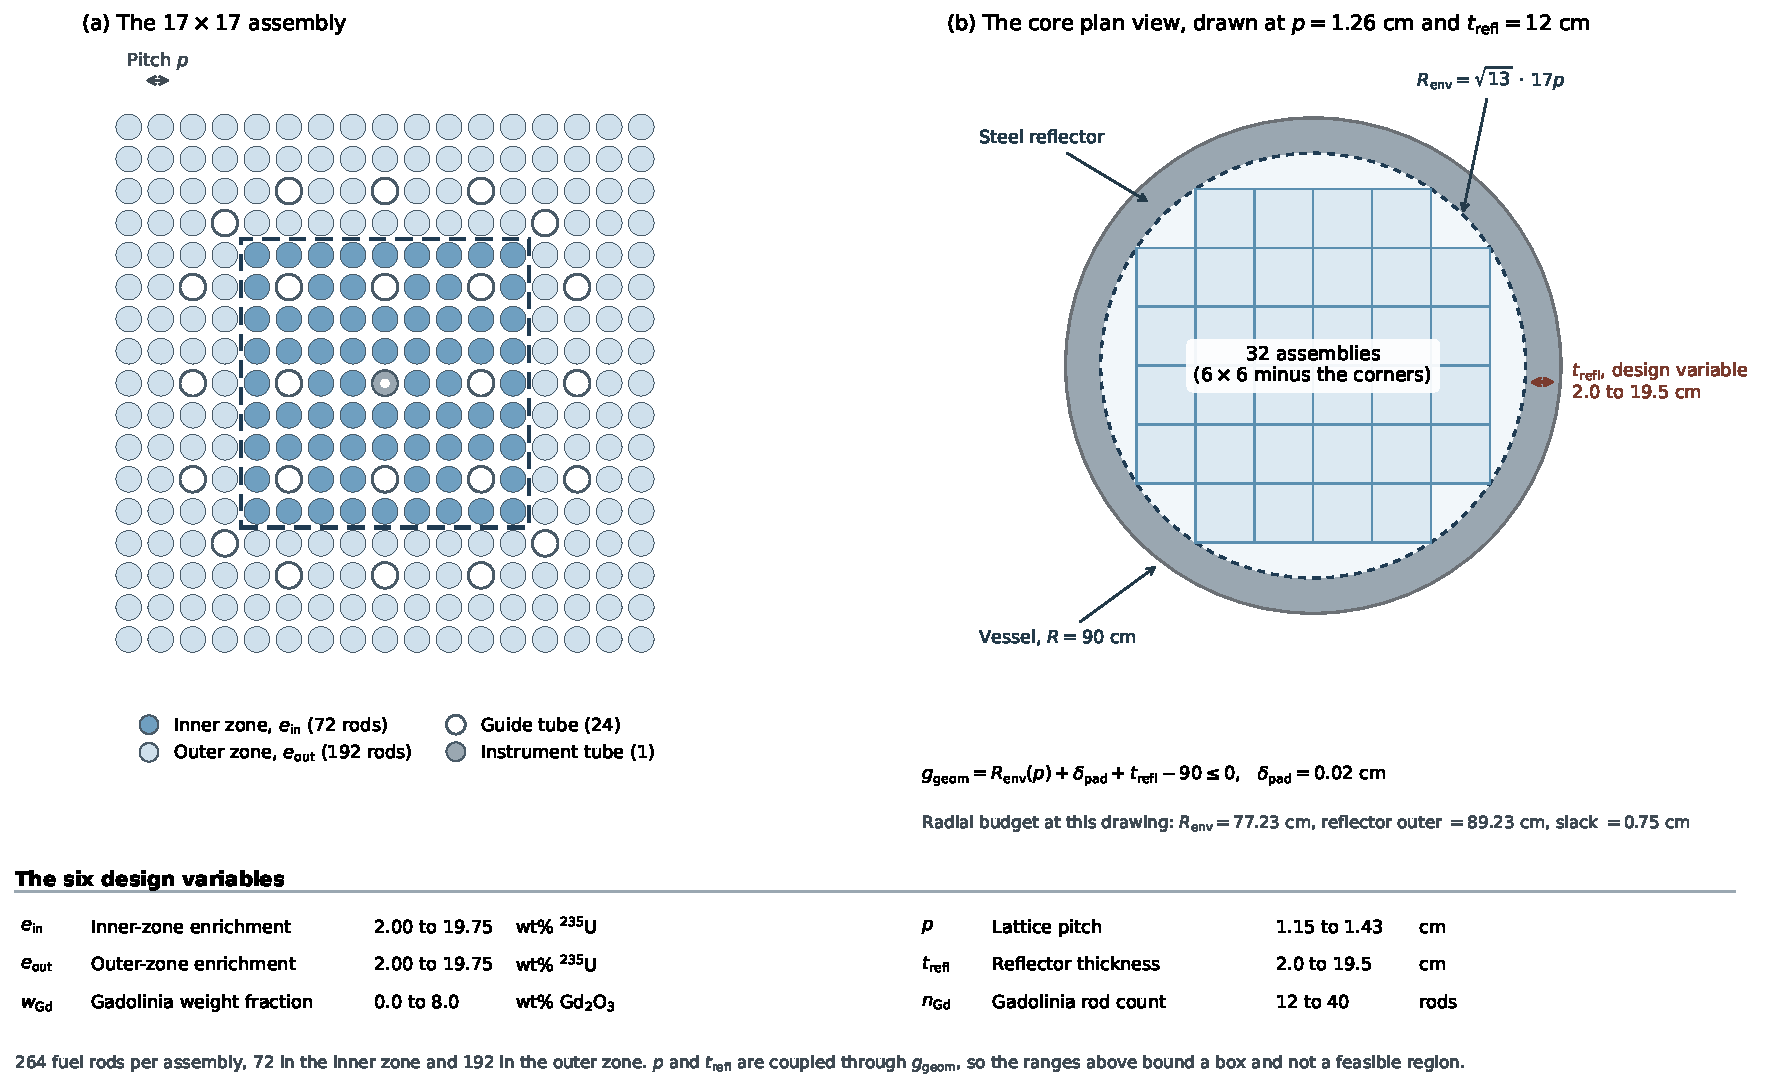
\includegraphics[width=\linewidth]{images/th_model_geometry.pdf}
  \caption[The reference model and the six-variable design space]{The reference model. (a)~The $17\times17$ assembly. (b)~The core plan view.}
  \label{fig:model-geometry}
\end{figure}

\begin{table}[htbp]
  \centering
  \caption{Geometry of the reference model.}
  \label{tab:model-geometry}
  \begin{tabular}{llc}
    \toprule
    Item & Value & Unit \\
    \midrule
    Fuel pellet outer radius & 0.406 & cm \\
    Cladding inner / outer radius & 0.414 / 0.475 & cm \\
    Guide-tube inner / outer radius & 0.572 / 0.612 & cm \\
    Lattice & $17\times17$: 264 rods, 24 GT, 1 IT & -- \\
    Inner enrichment zone & centred $9\times9$: 72 fuel rods (27\%) & -- \\
    Outer enrichment zone & 192 fuel rods (73\%) & -- \\
    Gd$_2$O$_3$ rods & 12 (C1--C4), discrete 12--40 (C5 on) & -- \\
    Active fuel height & 120 (heavy-metal mass only) & cm \\
    Core map & $6\times6$ minus corners = 32 assemblies & -- \\
    Reflector & stainless steel annulus, thickness $t_\mathrm{refl}$ & -- \\
    Vessel internal radius & 90 & cm \\
    \bottomrule
  \end{tabular}
\end{table}

The vessel internal radius is the 900\,mm inner radius of the simplified
vessel model dimensioned according to CTMSP~\cite{maruyama_2013}, as
detailed in Figure~\ref{fig:vessel-dimensioned}. The pin
and guide-tube dimensions follow NuScale-class
practice~\cite{nuscale_htp2_2017}. The core thermal power is the
48\,MW of thermal power that the Navy gives for the LABGENE
reactor~\cite{demartini_nuclep_2022}, within the 48 to 50\,MWth of the
academic literature~\cite{dinizcosta_2017}. The active height, the
enrichment zoning, the poisoned-pin pattern, the core map, the
reflector, the temperatures, the soluble boron concentration and the
nuclear data are modelling choices of this thesis.

\begin{table}[htbp]
  \centering
  \caption{Operating and material basis of the reference model.}
  \label{tab:model-operating}
  \begin{tabular}{llc}
    \toprule
    Item & Value & Unit \\
    \midrule
    Core thermal power & 48 & MW \\
    Specific power $P_\mathrm{spec}$ & 9.9834 & W/gHM \\
    Fuel / clad / moderator temperature & 900 / 600 / 580 & K \\
    Soluble boron (fixed, Sec.~\ref{sec:meth-boron}) & 1000 & ppm \\
    Nuclear data & ENDF/B-VII.1 + PWR chain & -- \\
    \bottomrule
  \end{tabular}
\end{table}

In three quantities the campaign model states its own value instead of
the one given by the reference specification. Each value is held fixed across the campaigns, so
that every design is evaluated on the same basis and the comparison
between designs is unaffected, and the effect of each on the absolute
result is measured in the three-dimensional confirmation.

\begin{enumerate}
  \item The heavy reflector is homogenised at \SI{90}{\%} steel by
        volume, a deliberately moderator-rich engineering estimate,
        against \SI{95.6}{\%} in the reference specification.

  \item The control rod absorber radius is \SI{0.433}{cm} for both
        absorbers, against \SI{0.423}{cm} for boron carbide and
        \SI{0.427}{cm} for silver-indium-cadmium in the reference specification.
        The clad radii, \num{0.4369} and \SI{0.484}{cm}, and the
        absorber number densities are those of the reference specification.

  \item The coolant density is \SI{0.72}{g/cm^3} at \SI{580}{K},
        against \SI{0.752}{g/cm^3} implied by the reference-specification number
        densities at its stated \SI{600}{K}. The boron mass fraction
        of \SI{1000}{ppm} is the same in both.
\end{enumerate}


\begin{figure}[htbp]
  \centering
  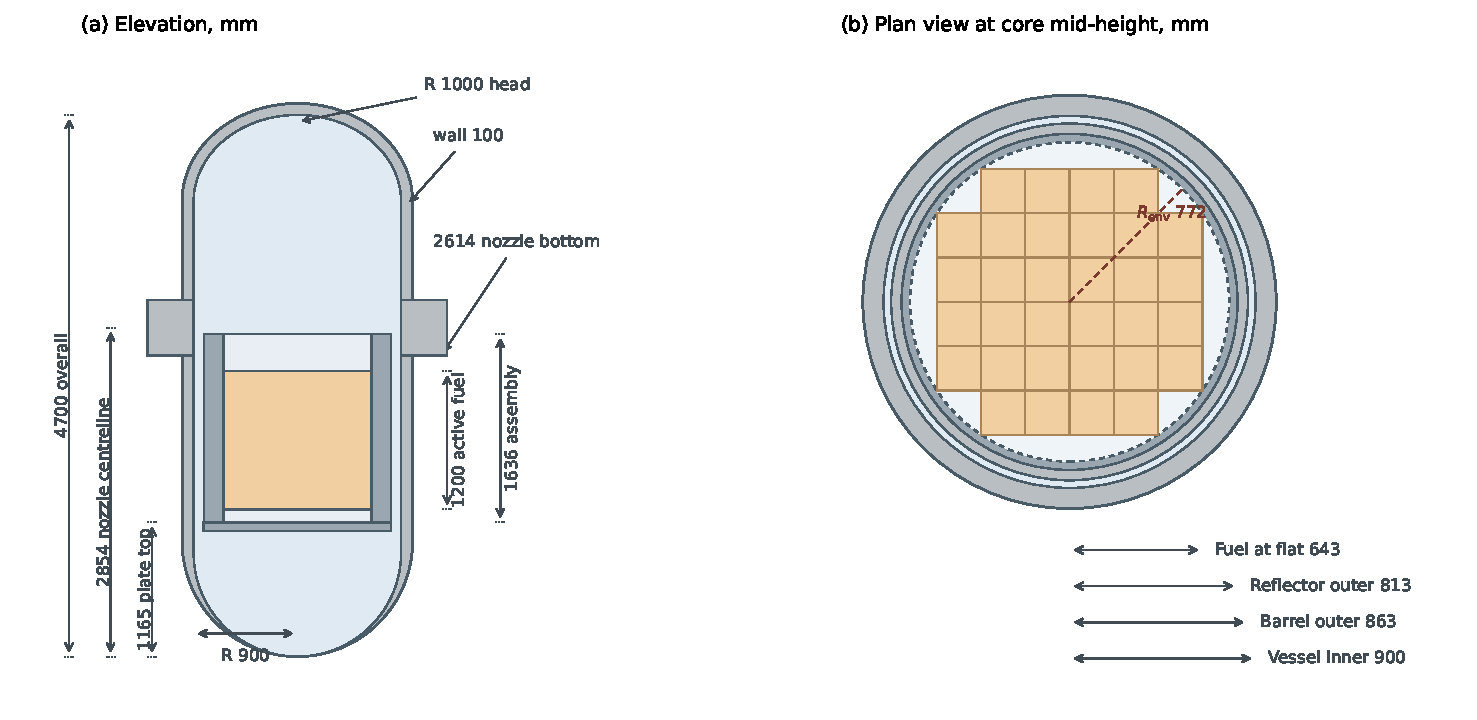
\includegraphics[width=\textwidth]{images/th_vessel_dimensioned}
  \caption{Elevation and plan view of the adopted vessel and core layout, in millimetres.}
  \label{fig:vessel-dimensioned}
\end{figure}

The dimensions of Figure~\ref{fig:vessel-dimensioned} have three
provenances, in the sense of the code table of
Table~\ref{tab:in-key}. The vessel envelope, with an overall height of 4700\,mm, a
cylindrical inner radius of 900\,mm, a wall thickness of 100\,mm and a
closure-head inner radius of 1000\,mm, is that of the simplified vessel
model dimensioned according to CTMSP~\cite{maruyama_2013}. The internal
elevations, the lower core plate and the coolant nozzle penetration,
were measured on that same drawing, which carries no dimension for
them, with the overall height as the scale reference, so they carry the
unquantified error of a graphical measurement. The structural components of the fuel assembly,
the nozzles, the end caps, the plenum spring and the spacer grids, keep
the sizes of the NuScale-like reference
specification~\cite{ez_aldeen_2025} without change.

The axial layout combines those two sources. The fixed components are
stacked above the lower core plate at their standard sizes, which
accounts for \SI{435.6}{mm} of the assembly, and the active fuel length
is the remainder up to the coolant nozzle penetration. That remainder is
\SI{1200}{mm}, against the \SI{2000}{mm} of the reference specification,
so the active length is set by the LABGENE-class envelope and not
inherited. The layout is therefore a standard fuel assembly, at
unchanged component sizes, fitted to the space this vessel leaves.

The active height of 120\,cm and the stainless steel reflector annulus
are modelling choices of this thesis, since no open source specifies the
reflector or the core barrel of LABGENE. The plan view of
Figure~\ref{fig:vessel-dimensioned} is constructed for a pin pitch of 1.26\,cm
and a minimum reflector thickness of 4.0\,cm.

\begin{figure}[htbp]
  \centering
  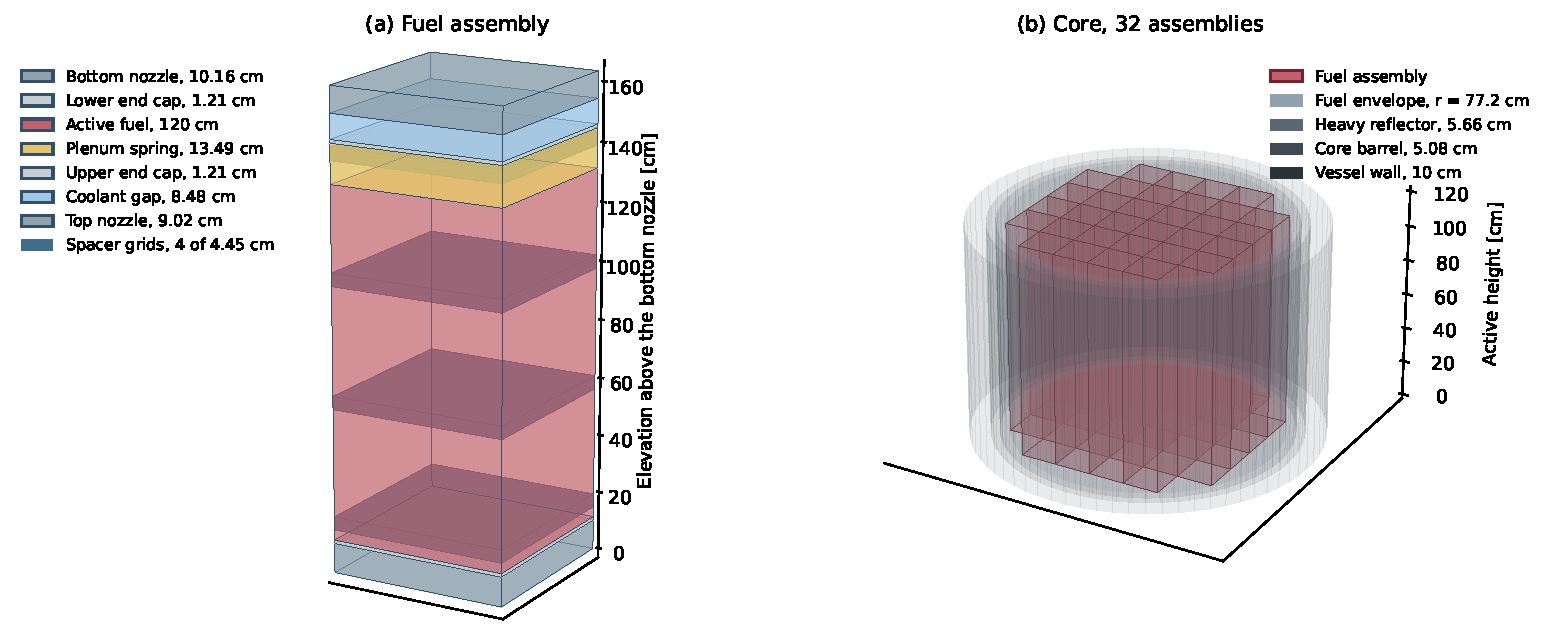
\includegraphics[width=\linewidth]{images/th_model_3d.pdf}
  \caption{The fuel assembly and the core in three dimensions.}
  \label{fig:model-3d}
\end{figure}

Figure~\ref{fig:model-3d} shows that assembly and the core in three
dimensions, and Table~\ref{tab:axial-layout} gives the axial layout
adopted for the three-dimensional core model. Elevations are measured
from the outer bottom of the lower head, with the assembly resting on
the lower core plate.

\begin{table}[htbp]
  \centering
  \caption{Axial layout of the fuel assembly in the three-dimensional core model, in millimetres.}
  \label{tab:axial-layout}
  \begin{tabular}{@{}lrrr@{}}
    \toprule
    \textbf{Item} & \textbf{Height} & \textbf{From} & \textbf{To} \\
    \midrule
    Bottom nozzle             &  101.6  & 1165.0 & 1266.6 \\
    Lower end cap             &   12.05 & 1266.6 & 1278.6 \\
    Active fuel               & 1200.0  & 1278.6 & 2478.6 \\
    Plenum spring             &  134.9  & 2478.6 & 2613.5 \\
    Upper end cap             &   12.05 & 2613.5 & 2625.6 \\
    Upper coolant gap         &   84.8  & 2625.6 & 2710.4 \\
    Top nozzle                &   90.2  & 2710.4 & 2800.6 \\
    \addlinespace
    Spacer grids, 4 of        &   44.45 & 1314.2 & 2600.8 \\
    \bottomrule
  \end{tabular}
\end{table}

The spacer grids take their materials and their height from the
reference specification, one of Inconel followed by three of Zircaloy.
Their number and their spacing do not follow it. The specification
carries five grids at a span of \SI{510.5}{mm} over \SI{2000}{mm} of
active fuel, whereas the shorter active length adopted here carries
four at an equal span of \SI{414}{mm}, of which three are inside the
active fuel and the fourth inside the plenum. The assembly is
\SI{1635.6}{mm} long.

\subsection{Treatment of the barrel and the downcomer in the campaign model}
\label{sec:meth-barrel}

The campaign transport model terminates in a vacuum boundary at the
outer surface of the heavy reflector, so the core barrel, the downcomer
water and the vessel wall of Figure~\ref{fig:vessel-dimensioned} carry
no transport solution. The radial space they occupy is still reserved
in the geometry, from Campaign 8 onward, by the vessel-fit constraint
of Equation~\eqref{eq:ggeom}, which holds the envelope of the core and
its reflector inside the \SI{90}{cm} vessel inner radius. No design is
therefore accepted that would leave those structures insufficient
radial clearance.

What the omission removes is the albedo of the region behind the
reflector, the fraction of the neutrons leaking from the reflector that
scatter back into the core. That albedo is set by materials and
thicknesses that are the same in every design, and it responds only
weakly to the design variables, so it raises every eigenvalue by nearly
the same amount, shifts every cycle length together and leaves the
ordering of the front unchanged. For the controllability constraint of
Section~\ref{sec:meth-ctrl} the omission acts in the non-conservative
direction. A vacuum boundary imposes zero albedo, so the modelled core
is less reactive than the real one in both rod states and the modelled
rodded core is more subcritical than the real one. That constraint acts on
the rodded eigenvalue itself rather than on a bank worth, so the albedo
does not cancel between the two states, and a design whose rodded
eigenvalue is close to the limit may pass the constraint while the real
geometry does not. The albedo is expected to be small, since the heavy
reflector already returns most of the neutrons that leave the core, and
the downcomer sensitivity of Section~\ref{sec:res-c8-3d}, in which the
downcomer is thinned from \SI{2.0}{cm} to \SI{3.7}{cm}, moves the
unrodded three-dimensional eigenvalue of design C8-47 by
\SI{-33}{pcm}. That bounds the sensitivity to the downcomer thickness
and not the albedo against a vacuum boundary, which was not quantified
in this work. The
three-dimensional confirmation model of Section~\ref{sec:res-c8-3d}
carries the barrel, the downcomer and the vessel wall explicitly, and
it introduces the axial leakage at the same time, so it does not
separate the two effects.

\section{Soluble boron treatment}
\label{sec:meth-boron}

The coolant carries a constant concentration of \SI{1000}{ppm} of
natural boron in every campaign of this work. The value is taken from
the operating conditions of the NuScale-like neutronics reference specification
defined by Fridman, Bilodid and
Valtavirta~\cite{fridman_nuscale_benchmark_2023}, together with the
uniform fuel temperature of \SI{900}{\kelvin} adopted in
Table~\ref{tab:model-operating}. The cladding and the steel structures
of that table are at \SI{600}{\kelvin}, and the coolant, which is also
the moderator, at \SI{580}{\kelvin}.

The concentration is a fixed modelling parameter, and no campaign of
this work exposes it to the optimiser as a design variable. Campaign 9 does carry a boron
quantity in its formulation, the critical concentration at the
operating maximum. That quantity is an objective, computed from each
evaluated design and minimised (Section~\ref{sec:meth-c9}), while the
depletion of that campaign still runs at the fixed \SI{1000}{ppm}.

The specification is static, at Beginning of Life (BOL), and does not
specify a depletion history. The extension of those
conditions to a depleted core is an assumption of the present work and
is treated as such in Section~\ref{sec:meth-boron-limits}.

\subsection{Basis for the choice}
\label{sec:meth-boron-basis}

Soluble boron is one of the reactivity-control methods of the boron-controlled
PWR lineage from which the present core
inherits its assembly geometry, and it is retained by the majority of
land-based light-water Small Modular Reactor (SMR) concepts now under
development. Four considerations support retaining it here.

\begin{enumerate}
  \item \textbf{Traceability of the reference conditions:} the
        NuScale-like reference specification provides a published
        input set, a
        Monte Carlo reference solution obtained with
        Serpent~\cite{fridman_nuscale_benchmark_2023}, and an
        independent reproduction with the same transport code and
        nuclear data library used in this work, namely OpenMC with
        ENDF/B-VII.1~\cite{ez_aldeen_2025}. That
        reproduction reports agreement within 16 to \SI{31}{pcm} in the
        effective multiplication factor and a root mean square relative
        difference below \SI{0.11}{\percent} in assembly radial power.
        No soluble boron specification for the LABGENE-class core that
        motivates the study is available in the open literature.
  \item \textbf{Containment of the design space:} soluble boron and the
        two absorber-related design variables, the gadolinium oxide
        (\ce{Gd2O3}) weight fraction and the gadolinium-bearing pin
        count, act on the same physical quantity, namely the excess
        reactivity available at beginning of life. Allowing boron to
        vary would make the study partly a study of boron rather than
        of the fuel and lattice variables under investigation.
  \item \textbf{Scope of the safety demonstration:} a
        Soluble-Boron-Free (SBF) core transfers the entire
        excess-reactivity budget to the burnable absorbers and the
        control rods, so its reactivity control rests on the control
        rod bank configuration. Three statements bound what this work
        establishes about that configuration.

        \begin{enumerate}[label=\theenumi.\arabic*, ref=\theenumi.\arabic*]
          \item \textbf{The configuration of the prototype is not
                available:} no open source gives the number of control
                rod banks of LABGENE, the assemblies each bank occupies,
                the absorber materials or the drive arrangement. The
                layout of Section~\ref{sec:meth-ctrl} is therefore an
                assumption of this work, taken from commercial PWR
                practice at the $17\times17$ guide-tube pattern.

          \item \textbf{The layout supports a first-order
                controllability check:} the constraint applied from
                Campaign 7 measures whether the reactivity worth that
                the regulating banks remove is large enough to hold the
                core subcritical at the states examined. It establishes
                the order of magnitude of the control requirement and
                rejects designs whose excess reactivity no credible bank
                could hold. It is not a shutdown margin.

          \item \textbf{A design configuration would need its own
                study:} fixing the banks would require a layout that
                meets the reactivity requirement at every state of the
                cycle and is mechanically achievable within the vessel
                head and the guide-tube pattern, together with a Cold
                Shutdown Margin (CSDM) demonstration under the
                single-failure assumption. That demonstration is outside
                the constraint set of every campaign.
        \end{enumerate}

        An SBF core adopted without that study would claim more than
        the present constraint set supports, so soluble boron is
        carried in every campaign of this work.
  \item \textbf{Known sign of the bias on the objective:} soluble
        boron absorbs part of the excess reactivity of the core, so a
        design evaluated with \SI{1000}{ppm} in the coolant reaches the
        end-of-cycle criterion of Equation~\eqref{eq:eoc} earlier than
        the same design would without boron. Every cycle length
        reported in this work is therefore a lower bound with respect
        to boron-free operation, and the sign of that bias is known
        without further calculation.
\end{enumerate}

Verification against a documented boron-controlled specification before
boron-free operation is addressed is established practice: Ez Aldeen et
al.~\cite{ez_aldeen_2025} adopt the same specification as the verification
basis of a study aimed at boron-free SMR cores.

Soluble-boron-free operation recurs in the compact and civil marine
light-water designs of the open literature, and its reported
motivations are reviewed in
Section~\ref{subsec:comparison}~\cite{kusunoki_mrx_2000,alam_partI_2019,alzaben_boronfree_2019,ismr_sbf_2024,rr_smr_atf_2025,song_sanchez_2026}.
Reactivity-control practice in operating naval propulsion reactors is
not documented in publicly available sources, and no claim about it is
made here.

%% labels of the material summarised in the boron section, kept so that the
%% cross-references of the other chapters still resolve
\label{sec:meth-boron-bias}\label{eq:boron-rho-to-k}

\subsection{Declared limitations}
\label{sec:meth-boron-limits}

\begin{enumerate}
  \item The specification from which the concentration is taken is static
        Beginning of Life (BOL) specification. Its extension to a
        depleted core is an assumption of the present work and is not
        supported by the specification itself.
  \item The concentration is held constant throughout depletion, and no
        critical boron search feeds back into it. Campaign 9 does search
        for the critical concentration, at beginning of life only, over
        the measured boron points of Section~\ref{sec:meth-c9}, and the
        concentration at the operating maximum is inferred from the
        gadolinium hump through Equation~\eqref{eq:c9-cmax} rather than
        searched. No search is performed at any later burnup step, so
        the depletion trajectory represents a reactivity-tracking model
        and not an operating history.
  \item The MTC is not evaluated inside the optimisation loop, so no
        design is rejected on it. It was measured only after Campaigns 8
        and 9, as the MTC boron limit of
        Section~\ref{sec:meth-mtc}, on one design and on eight candidate
        lattices respectively, and each candidate was then compared
        against its own limit. The limit rises with the gadolinia
        loading, so it is a property of the design, and the values are
        reported in Section~\ref{sec:res-c9-ceiling}.
  \item Boron depletion and \isotope[10]{B} burnout are not modelled,
        which is consistent with the constant-concentration assumption.
\end{enumerate}

%% labels of the material reported in the results, kept so that the
%% cross-references of the other chapters still resolve
\label{sec:meth-boron-worth}\label{eq:rho-def}\label{eq:boron-worth}\label{eq:rod-only-margin}\label{eq:boron-share}

\section{Optimisation problem}
\label{sec:meth-problem}

\subsection{Problem statement}

The core design is formulated as a constrained two-objective
optimisation problem over a design space of four to six decision
variables, depending on the campaign (Tables~\ref{tab:design-space}
and~\ref{tab:c89-spec}). The constraints are summarised in
Table~\ref{tab:constraints}.

The first objective maximises the cycle length.

\begin{equation}
\max_{\mathbf{x}\,\in\,\mathcal{X}} \, \mathrm{EFPD}(\mathbf{x})
\label{eq:obj_efpd}
\end{equation}

The second objective minimises the radial peaking factor.

\begin{equation}
\min_{\mathbf{x}\,\in\,\mathcal{X}} \, F_{\Delta H}(\mathbf{x})
\label{eq:obj_fdh}
\end{equation}

This pair of objectives is the one of Campaigns 1 to 8. Campaign 9 keeps
the peaking objective and the evaluator of Campaign 8, and changes the
other half of the problem:

\begin{itemize}
  \item The cycle length leaves the objectives and becomes a constraint
        at the required five years.

  \item The critical boron concentration at the most reactive state of
        the cycle becomes the second objective, so both objectives are
        minimised.
\end{itemize}

Equation~\eqref{eq:c9-problem} in Section~\ref{sec:meth-c9} states that
formulation. The design space is fixed from Campaign 8 onwards, with the
pitch held at \SI{1.26}{cm} and a design vector of four components
against the six of the earlier campaigns
(Section~\ref{sec:meth-c8-space}).

Both are subject to the feasibility condition below.

\begin{equation}
g_j(\mathbf{x}) \le 0,
\qquad j = 1,\dots,n_g
\label{eq:constraint_form}
\end{equation}

\noindent where the symbols have the following meaning.

\begin{itemize}
  \item $\mathbf{x}$ is the design vector, whose components and their
        units are listed in Tables~\ref{tab:design-space}
        and~\ref{tab:c89-spec}. It has five components in Campaigns 1
        to 4, six in Campaigns 5 to 7, and four in Campaigns 8 and 9.

  \item $\mathcal{X}$ is the box-bounded design space defined by those
        same bounds.

  \item $\mathrm{EFPD}(\mathbf{x})$ is the cycle length of design
        $\mathbf{x}$ in effective full-power days, obtained from
        Equation~\eqref{eq:efpd} with the end-of-cycle criterion of
        Section~\ref{sec:objective_functions}.

  \item $F_{\Delta H}(\mathbf{x})$ is the radial peaking factor of
        design $\mathbf{x}$, dimensionless, defined in
        Equation~\eqref{eq:fdh_definition}.

  \item $g_j(\mathbf{x})$ is the $j$-th inequality constraint of
        Table~\ref{tab:constraints}, expressed in its own native unit
        and feasible when non-positive. The normalisation applied
        before the constraints are aggregated to rank infeasible
        populations is introduced in Campaign 6 and defined in
        Equation~\eqref{eq:cv-norm}.

  \item $n_g$ is the number of active inequality constraints,
        dimensionless: four in Campaign 1, five in Campaigns 2 to 6,
        six in Campaigns 7 and 8 and eight in Campaign 9
        (Table~\ref{tab:constraints}). The two-bank reading
        $g_\mathrm{ctrl,12}$ and the boron record $g_\mathrm{boron}$ of
        Campaign 9 are recorded and not constrained.
\end{itemize}

The transport model on which $F_{\Delta H}$ is evaluated changes between
campaigns and is
fixed in Section~\ref{sec:objective_functions}, with the validation
that motivated the change in Section~\ref{sec:meth-core-objective}.

Table~\ref{tab:design-space} gives the design variables and their
bounds up to Campaign 7.

\begin{itemize}
  \item $e_\mathrm{in}$ and $e_\mathrm{out}$, the enrichments of the
        inner and outer zones of the assembly.

  \item $w_\mathrm{Gd}$, the Gd$_2$O$_3$ weight fraction in the
        poisoned rods.

  \item $p$, the pin pitch.

  \item $t_\mathrm{refl}$, the reflector thickness.

  \item $n_\mathrm{Gd}$, the number of gadolinia rods, added as a sixth
        variable in Campaign 5.
\end{itemize}

Three campaigns then change the bounds.

\begin{itemize}
  \item Campaign 6 lowers the enrichment bound to the value implied by
        the zoned low-enriched-uranium limit of
        Section~\ref{sec:meth-zoning}.

  \item Campaign 7 narrows the enrichment box to
        $12/1.150 = \SI{10.43}{wt\%}$ by Equation~\eqref{eq:leu-box},
        from the limit on the peripheral ring lowered to
        \SI{12}{wt\%}, and sets a lower bound of \SI{3.0}{wt\%} as a
        exploratory choice.

  \item Campaign 9 returns that lower bound to \SI{2.0}{wt\%}.
\end{itemize}

The design space of Campaigns 8 and 9 is given in
Table~\ref{tab:c89-spec}.

\begin{table}[htbp]
  \centering
  \small
  \caption{Design variables and bounds, Campaigns 1 to 7.}
  \label{tab:design-space}\label{tab:design-space-c56}\label{tab:design-space-c78}
  \begin{tabular}{@{}llcccc@{}}
    \toprule
    Variable & Unit & C1--C4 & C5 & C6 & C7 \\
    \midrule
    $e_\mathrm{in}$, $e_\mathrm{out}$ & wt\% $^{235}$U & 2.0--19.75 & 2.0--19.75 & 2.0--17.174 & 3.0--10.43 \\
    $w_\mathrm{Gd}$ & wt\% & 0--8.0 & 0--8.0 & 0--8.0 & 0--8.0 \\
    $p$ & cm & 1.15--1.43 & 1.15--1.43 & 1.15--1.43 & 1.15--1.43 \\
    $t_\mathrm{refl}$ & cm & 2.0--19.5 & 2.0--19.5 & 2.0--19.5 & 2.0--19.5 \\
    $n_\mathrm{Gd}$ & rods & 12, fixed & 12--40 & 12--40 & 12--40 \\
    \bottomrule
  \end{tabular}
\end{table}

Figure~\ref{fig:gd-ladder} illustrates the six nested patterns of
Table~\ref{tab:design-space}, each panel showing the pins inherited
from the next lower rod count and the pins added at that count.

\begin{figure}[htbp]
  \centering
  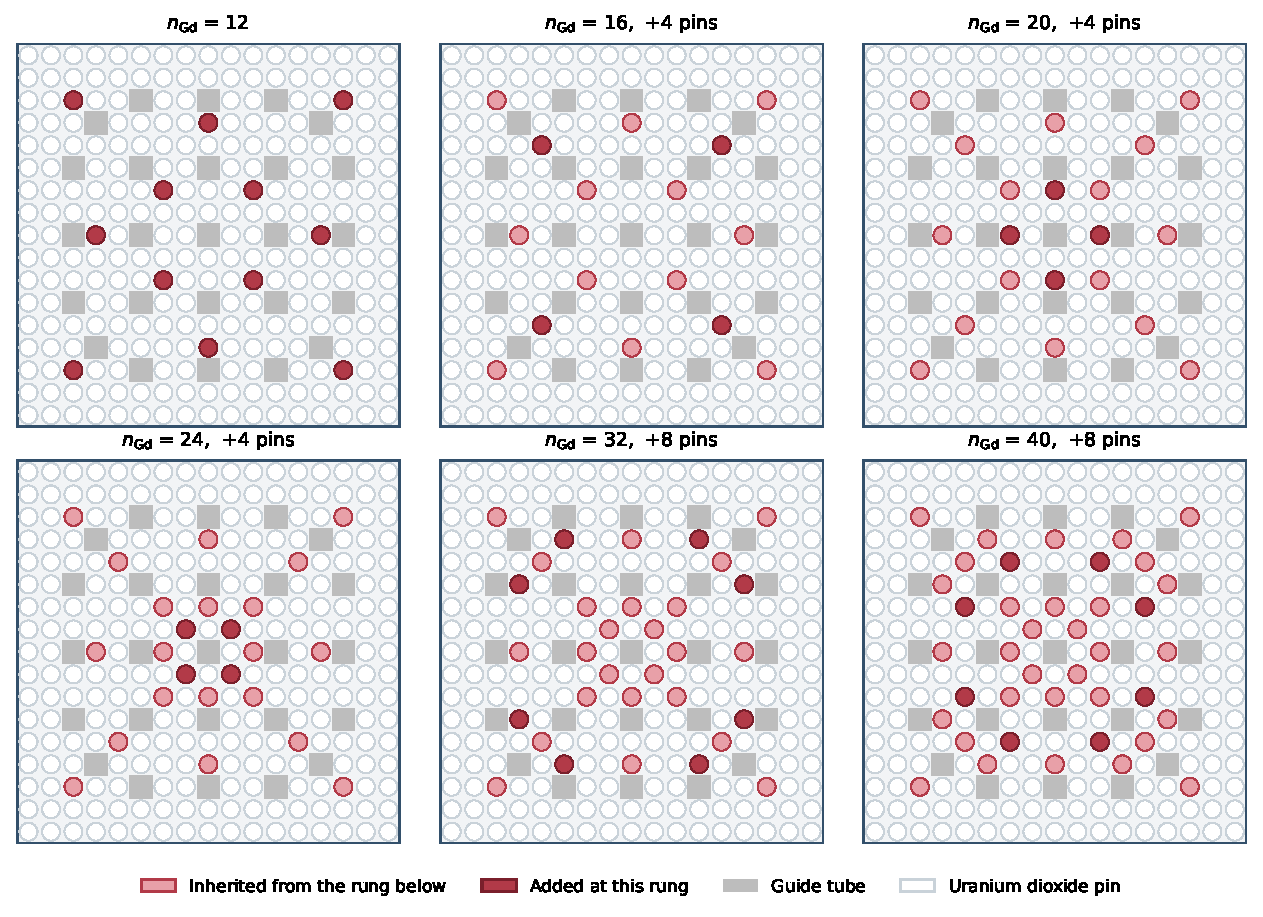
\includegraphics[width=0.92\linewidth]{images/th_gd_ladder.pdf}
  \caption{The six nested poisoned-pin patterns.}
  \label{fig:gd-ladder}
\end{figure}

The rod count is a discrete variable, and it reaches the model in three
steps:

\begin{enumerate}
  \item NSGA-II treats the pin count as a continuous variable inside
        the bounds, so it proposes values such as 13.845.

  \item The evaluator snaps that value to the nearest admissible
        rod count, one of 12, 16, 20, 24, 32 and 40, before the model
        is built, and an exact midpoint is assigned to the lower count.

  \item The archive records both numbers, the value the optimiser
        proposed and the value that was built.
\end{enumerate}

In Campaign 9, for example, the design of index 0 was proposed at
13.845 pins and built with 12, and the design of index 2 was proposed
at 22.446 and built with 24. The positions the added rods take are not free. A gadolinia rod
depresses the thermal flux around itself, so where the rods are placed
changes the assembly peaking factor and the burnout rate of the
absorber at the same rod count. The placement strategy therefore puts
each new rod in the interior of the assembly, around the guide tubes,
following
the optimised 16, 20 and 24 pin maps of Bae, Mertyurek and
Asgari~\cite{bae_gd_2023} and the arrangements of the reference
specification~\cite{nuscale_htp2_2017,epr_fsar_ch4}, under four rules.

\begin{enumerate}
  \item The patterns are nested, so each contains the one below it and
        the twelve-rod heritage arrangement of Campaigns 1 to 4 is the
        smallest of them.
  \item Every pattern is octant-symmetric.
  \item The outer two rod rows are kept absorber free.
  \item Every gadolinia rod is face-adjacent or diagonally adjacent to
        a guide tube, and no two gadolinia rods are face-adjacent to
        each other, which limits mutual shadowing.
\end{enumerate}

\begin{table}[htbp]
  \centering
  \small
  \caption{Constraints: definition and transport model of evaluation.}
  \label{tab:constraints}
\begin{tabularx}{\textwidth}{
    >{\raggedright\arraybackslash}p{0.15\textwidth}
    >{\raggedright\arraybackslash}p{0.40\textwidth}
    >{\raggedright\arraybackslash}X
}
    \toprule
    Constraint & Definition & Evaluated on \\
    \midrule
    $g_{k\min}$ 
        & $1.02 - k_\mathrm{BOL} \le 0$
        & assembly to C5, \textbf{core} from C6 \\

    $g_{k\max}$ 
        & $k_\mathrm{BOL} - k_{\max} \le 0$
        & assembly to C5, \textbf{core} from C6, 
          $k_{\max}$ of Table~\ref{tab:ctrl-bounds} \\

    $g_\mathrm{enr}$ 
        & $e_\mathrm{zoned,max} - e_\mathrm{lim} \le 0$
        & algebraic, $e_\mathrm{lim}$ per campaign \\

    $g_\mathrm{peak}$ 
        & $F_{\Delta H} - 2.0 \le 0$
        & assembly in C1 to C3, \textbf{core} from C4 \\

    $g_\mathrm{geom}$ 
        & $R_\mathrm{env}(p) + \delta + t_\mathrm{refl} + c_\mathrm{v} - 90 \le 0$
        & core, analytic, lattice pad $\delta$ of
          Equation~\eqref{eq:ggeom}, clearance $c_\mathrm{v}$ of 
          Section~\ref{sec:meth-c8-space} \\

    $g_\mathrm{ctrl}$ 
        & $k_\mathrm{RE} - 0.99 \le 0$
        & \textbf{core}, the sixteen regulating-bank assemblies in,
          from C7 \\

    $g_\mathrm{ctrl,12}$ 
        & $k_\mathrm{RE12} - 0.99$
        & core, first two banks in, from C8, 
          \emph{recorded, not constrained} \\
    \bottomrule
\end{tabularx}
\end{table}

The bound of $g_\mathrm{peak}$ takes two values. Campaigns 1 to 8 use
2.0, a deliberately generous adopted value that keeps the exploratory
search free~\cite{epr_fsar_ch4}, and Campaign 9 uses 1.65, the
Technical Specification limit of a licensed pressurised water
reactor~\cite{robinson_gd10}, for the reason given in
Section~\ref{sec:meth-c9}. Satisfying either value is a necessary
condition on a candidate design and not a demonstration of compliance.

\subsection{Geometric feasibility}
\label{sec:meth-geom}

The vessel-fit constraint $g_\mathrm{geom}$ uses the circumscribed
envelope of the intact core footprint.

\begin{equation}
R_\mathrm{env}(p) = \sqrt{13}\,\cdot\,17\,p
\label{eq:renv}
\end{equation}

\noindent where the symbols have the following meaning.

\begin{itemize}
  \item $R_\mathrm{env}$ is the circumscribed radius of the fuel
        region, in cm.

  \item $p$ is the pin pitch, in cm.

  \item $17$ is the number of pin cells per assembly side,
        dimensionless, so that $17p$ is the assembly pitch in cm.

  \item $\sqrt{13} \approx 3.606$ is the dimensionless distance from
        the core centre to the outermost fuel corner of the
        $6\times6$-minus-corners map, in assembly pitches. The extreme
        corner is three assembly pitches along one axis and two along
        the other, so its distance is $\sqrt{3^2 + 2^2} = \sqrt{13}$.
\end{itemize}

The sensitivity of the envelope to the pitch follows directly.

\begin{equation}
\frac{\mathrm{d}R_\mathrm{env}}{\mathrm{d}p} = 61.3~\mathrm{cm\,cm^{-1}}
\label{eq:drenv}
\end{equation}

A pitch increase of one millimetre therefore consumes about
\SI{6.1}{cm} of radial budget. Pitch and reflector thickness compete
directly for the fixed allowance of the 90\,cm vessel internal radius
of Table~\ref{tab:model-geometry}, which makes the two variables
strongly coupled.

The enforced form of the constraint carries two further terms. The
geometry builder pads the lattice corner by a fixed allowance, and
Campaign 8 reserves a clearance for the core barrel and the downcomer.
\begin{equation}
g_\mathrm{geom} \;=\; R_\mathrm{env}(p) \;+\; \delta \;+\;
t_\mathrm{refl} \;+\; c_\mathrm{v} \;-\; R_\mathrm{v} \;\le\; 0
\label{eq:ggeom}
\end{equation}

\noindent where the symbols have the following meaning.

\begin{itemize}
  \item $R_\mathrm{env}(p)$ is the circumscribed radius of
        Equation~\eqref{eq:renv}, in cm.

  \item $\delta$ is the lattice-corner pad of the geometry builder,
        \SI{0.02}{cm}, held in a single constant shared by the builder
        and the constraint.

  \item $t_\mathrm{refl}$ is the reflector thickness, in cm.

  \item $c_\mathrm{v}$ is the reserved barrel and downcomer clearance,
        in cm. It is zero in Campaigns 1 to 7 and \SI{7.08}{cm} in
        Campaigns 8 and 9, as derived in
        Section~\ref{sec:meth-c8-space}. Campaign 9 keeps it, so both
        campaigns search the reflector thickness up to the same
        \SI{5.66}{cm}.

  \item $R_\mathrm{v}$ is the vessel internal radius, \SI{90}{cm}.
\end{itemize}

The pad $\delta$ of \SI{0.02}{cm} is the allowance the geometry builder
adds at the lattice corner so that the outermost pin cells close inside
the core envelope. The builder has applied it from the first campaign.
The analytic constraint did not, up to and including Campaign 4, so the
envelope the optimiser tested was \SI{0.02}{cm} smaller than the one the
code then built.

That difference is only reached by a design whose reflector stands
within \SI{0.02}{cm} of the vessel limit, and the search produces such
designs by construction, since a thicker reflector returns more neutrons
and the optimiser pushes the reflector thickness against its upper bound
wherever reactivity is the binding objective. The first infill batch of
Campaign 4 proposed one, the constraint accepted it, and the geometry
builder could not construct it, so the evaluation failed. The pad is now
a single constant imported by both the constraint and the builder, so
the two descriptions of the same core cannot differ again.

The constraint is tested analytically inside the optimiser, before any
geometry is built, so a design that cannot fit the vessel is rejected
without spending a transport evaluation on it.

\subsection{Eigenvalue model of the reactivity window}
\label{sec:meth-kbasis}

Campaigns 1 to 5 applied the reactivity window to the assembly infinite
multiplication factor. From Campaign 6 both of its bounds act on the
core effective multiplication factor at beginning of life, which the
leakage-corrected target of Section~\ref{sec:meth-ktarget} makes
available at no additional cost, for the reason reported in
Section~\ref{sec:res-c4}. The upper bound is not a constant of this work. It
is the adopted value up to and including Campaign 6 and a
derived quantity from Campaign 7 onwards, so it is written here as a symbol.

\begin{equation}
1.02 \;\le\; k_\mathrm{eff}^\mathrm{core}(\mathbf{x}) \;\le\; k_{\max}
\label{eq:k-window-core}
\end{equation}

\noindent where the symbols have the following meaning.

\begin{itemize}
  \item $k_\mathrm{eff}^\mathrm{core}$ is the effective multiplication
        factor of the 32-assembly core at the beginning of life,
        dimensionless, from the same core solve on which the peaking
        objective is tallied.

  \item $\mathbf{x}$ is the design vector of
        Table~\ref{tab:design-space}.

  \item $k_{\max}$ is the upper reactivity bound of the campaign,
        dimensionless. It is 1.35 through Campaign 6 and takes the
        derived values of Table~\ref{tab:ctrl-bounds} from Campaign 7,
        namely 1.126 in Campaign 7 and 1.166 in Campaigns 8 and 9.
\end{itemize}

The change of basis affects the two bounds differently.

The upper bound keeps the same feasible set. Re-scored on both bases, the
Campaign 5 archive admits the same designs with the core bound at 1.35
as with the assembly bound at 1.40
(Section~\ref{sec:res-c5-kbasis}), so the problem is no looser than
before.

The floor becomes active. The assembly is solved under reflective
boundary conditions, which return every neutron, so its $k_\infty$
carries no leakage and a floor of 1.02 on it rejects almost no design.
The core eigenvalue carries the radial and axial leakage of the whole
core, is therefore several thousand pcm lower for the same design, and
the same floor of 1.02 now rejects the designs that cannot reach
criticality. Campaign 6 shows that happening repeatedly
(Section~\ref{sec:res-c6-doe}).

\subsection{controllability constraint and the upper reactivity bound}
\label{sec:meth-ctrl}

In Campaigns 1 to 6 the upper bound of the reactivity window is an
adopted value of 1.35 and not a controllability criterion.
The transport model of those campaigns carries no control rods, no
rodded state is solved and no bank worth enters the constraint set. The
value bounds the excess reactivity the search may accumulate while the
objective is the cycle length, which is what the exploratory phase
needs.

Controllability is assessed for the first time in the post-analysis of
the Campaign 6 archive, on the first front of this work whose designs
are worth examining as candidates. That assessment produced the
seven-bank scheme of Figure~\ref{fig:cr-banks} and the constraint below,
which enter the constraint set in Campaign 7 under the one-change rule
of Section~\ref{sec:meth-campaigns}.

The constraint replaces the adopted value by a measurement. Every
evaluation of Campaign 7 solves the beginning-of-life core twice, and
every evaluation of Campaigns 8 and 9 three times:

\begin{enumerate}
  \item With every bank withdrawn, which gives the peaking objective
        and the unrodded eigenvalue.

  \item With the four regulating banks inserted, which gives
        $k_\mathrm{RE}$, the eigenvalue the constraint acts on.

  \item From Campaign 8, with the first two regulating banks inserted,
        which gives $k_\mathrm{RE12}$. That reading is recorded and not
        constrained, and it divides the front as described below.
\end{enumerate}

Every assembly of the core carries a control rod assembly, so the
state with all 32 inserted bounds what the control system can hold. The
constraint is conservative with respect to that bound, because it inserts
only the four regulating banks and leaves the shutdown banks
withdrawn.

The banks are those of the seven-bank scheme illustrated in
Figure~\ref{fig:cr-banks}. The scheme was not applied in Campaign 6. It
was defined in the post-analysis of the Campaign 6 archive and entered
the constraint set from Campaign 7, so it governs Campaigns 7, 8 and 9
only. The regulating banks RE1 to RE4
occupy the sixteen central assemblies and carry B$_4$C absorbers. The
shutdown banks occupy the outer sixteen assemblies and stay withdrawn
throughout, because they are reserved for the scram function and a
design that needs them at power is not controllable in normal
operation.

\begin{figure}[htbp]
  \centering
  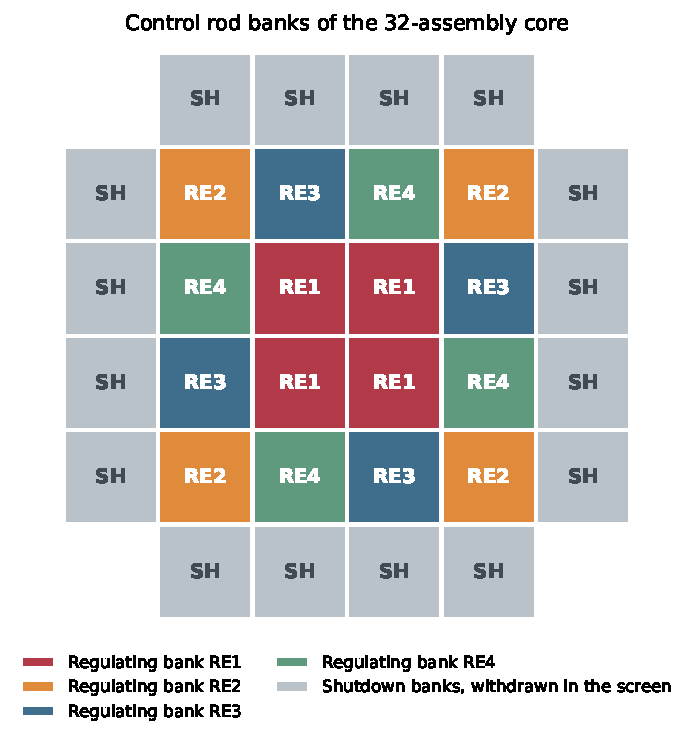
\includegraphics[width=0.62\linewidth]{images/th_cr_banks.pdf}
  \caption{Control rod banks of the 32-assembly core.}
  \label{fig:cr-banks}
\end{figure}

\begin{equation}
k_\mathrm{RE}(\mathbf{x}) = k_\mathrm{eff}^\mathrm{core}\big(\mathbf{x},\ \mathrm{RE1\ to\ RE4\ inserted}\big)
\label{eq:k-re}
\end{equation}

\noindent where the symbols have the following meaning.

\begin{itemize}
  \item $k_\mathrm{RE}$ is the core effective multiplication factor at
        beginning of life with the sixteen regulating-bank assemblies
        inserted and the sixteen shutdown-bank assemblies withdrawn,
        dimensionless.

  \item $\mathbf{x}$ is the design vector.
\end{itemize}

The constraint demands an operating subcriticality margin.

\begin{equation}
g_\mathrm{ctrl}(\mathbf{x}) = k_\mathrm{RE}(\mathbf{x}) - (1 - \Delta\rho_\mathrm{op}) \le 0
\label{eq:g-ctrl-meth}
\end{equation}

\noindent where the symbols have the following meaning.

\begin{itemize}
  \item $g_\mathrm{ctrl}$ is the constraint value, dimensionless,
        negative when satisfied.

  \item $\Delta\rho_\mathrm{op}$ is the operating margin, \num{0.01} in
        units of $k$, that is \SI{1000}{pcm}.
\end{itemize}

The worth of the regulating banks is read from the same pair of solves.

\begin{equation}
\rho_\mathrm{bank}(\mathbf{x}) = k_\mathrm{eff}^\mathrm{core}(\mathbf{x}) - k_\mathrm{RE}(\mathbf{x})
\label{eq:bank-worth}
\end{equation}

\noindent where the symbols have the following meaning.

\begin{itemize}
  \item $\rho_\mathrm{bank}$ is the worth of the sixteen regulating-bank
        assemblies, in units of $k$, reported in pcm after
        multiplication by $10^5$.

  \item $k_\mathrm{eff}^\mathrm{core}$ is the unrodded core effective
        multiplication factor at beginning of life, dimensionless.
\end{itemize}

The margin is a modelling choice. An insertion of the regulating banks
alone with a \SI{1000}{pcm} margin is not a licensing shutdown
margin. The constraint
therefore tests whether the regulating system can hold the fresh core
subcritical at power conditions, which is the question the reactivity
bound was standing in for.

Two further rodded states appear in this work, and neither is
constrained. The state $k_\mathrm{RE12}$ inserts only the eight
assemblies of banks RE1 and RE2, the four central assemblies and the
four diagonal assemblies of the middle ring. It is recorded from
Campaign 8 as $g_\mathrm{ctrl,12}$, so that the post-analysis can
divide the front into designs controllable with two banks and designs
that need all four. The margins $M_{16}$ and $M_{8}$ of
Table~\ref{tab:c8-post-boron} are those of the sixteen- and of the
eight-assembly insertion. Neither is a margin of the all-rods-in state,
which inserts all 32 control rod assemblies and therefore includes the
sixteen shutdown-bank assemblies that this work keeps
withdrawn.

The upper reactivity bound of $g_{k\max}$ can now be derived from the
measured bank worth rather than adopted.

\begin{equation}
k_{\max} = (1 - \Delta\rho_\mathrm{op}) + \min_{\mathbf{x} \in \mathcal{S}} \rho_\mathrm{bank}(\mathbf{x})
\label{eq:k-max-derived}
\end{equation}

\noindent where the symbols have the following meaning.

\begin{itemize}
  \item $k_{\max}$ is the derived bound on the unrodded core
        eigenvalue, dimensionless.

  \item $\rho_\mathrm{bank}$ is the bank worth, the difference between
        the unrodded and the rodded eigenvalues, dimensionless.

  \item $\mathcal{S}$ is the sample of designs on which the worth was
        measured.
\end{itemize}

Table~\ref{tab:ctrl-bounds} lists the bounds used and derived. Its
three-dimensional values come from the axial study of
Section~\ref{sec:meth-lax}.

\begin{table}[htbp]
  \centering
  \caption{Upper reactivity bounds by campaign and their provenance.}
  \label{tab:ctrl-bounds}
  \small
  \begin{tabularx}{\textwidth}{@{}>{\raggedright\arraybackslash}p{0.16\textwidth}c>{\raggedright\arraybackslash}p{0.20\textwidth}>{\raggedright\arraybackslash}X@{}}
    \toprule
    Campaigns & $k_{\max}$ & Basis & Provenance \\
    \midrule
    C1 to C6 & 1.35  & assembly, then core & adopted value \\
    retrospective & 1.368 & core, 2D & all seven banks, \SI{1000}{pcm}, eight C6 designs \\
    C7 & 1.126 & core, 2D & four regulating banks, eight C6 designs, worths \num{12174} to \SI{12718}{pcm} \\
    C7 measured & 1.099 to 1.217 & core, 2D & implied by each design's own worth, 60 designs \\
    C8 and C9 & 1.166 & core, 2D from 3D & smallest 3D worth \SI{14307}{pcm}, times $L_\mathrm{ax}$ \\
    \bottomrule
  \end{tabularx}
\end{table}

A bound derived this way has two weaknesses. The minimum of a small
sample is a biased estimate of the minimum of the population, and the
quantity it stands in for is measured on every evaluation from Campaign
7. From Campaign 8 the measured constraint therefore decides feasibility,
and the derived value is kept only as a outer bound
(Section~\ref{sec:res-c7-screens}).

The retrospective value of 1.368, derived from the worth of all 32
control rod assemblies with the same margin, is two per cent above the
adopted 1.35, which is therefore the all-bank controllability bound of
this core to within that tolerance.


\subsection{Objective functions}
\label{sec:objective_functions}

\subsubsection{Cycle length}

The cycle length is an objective in Campaigns 1 to 8 and a constraint in
Campaign 9, where the five-year requirement enters
Equation~\eqref{eq:c9-problem}. It is computed in the same way in both
cases, from the end-of-cycle burnup through the conversion of
Equation~\eqref{eq:efpd}, with the specific power of
Table~\ref{tab:model-operating}. What remains to be fixed here is the
criterion that defines the end of cycle on the model used for the
depletion, the reflective single assembly.

\begin{equation}
B_\mathrm{EOC} = \min\!\left( B_k,\, B_\mathrm{burnup} \right)
\label{eq:eoc}
\end{equation}

\begin{equation}
B_k = \min\left\{\, B > 0 \,:\, k_\infty(B) \le k_\mathrm{target} \,\right\}
\label{eq:eoc-k}
\end{equation}

\noindent where the symbols have the following meaning.

\begin{itemize}
  \item $B_\mathrm{EOC}$ is the end-of-cycle burnup entering
        Equation~\eqref{eq:efpd}, in MWd/kgHM.

  \item $B_k$ is the reactivity-defined end-of-cycle burnup, in
        MWd/kgHM.

  \item $B_\mathrm{burnup}$ is the discharge-burnup limit, equal to
        55\,MWd/kgHM on the assembly-average basis, with its basis and
        its relation to the depletion horizon in
        Section~\ref{sec:meth-atf}.

  \item $B$ is the burnup along the depletion history, in MWd/kgHM.

  \item $k_\infty(B)$ is the infinite multiplication factor of the
        reflective assembly at burnup $B$, dimensionless.

  \item $k_\mathrm{target}$ is the leakage-corrected end-of-cycle
        target, dimensionless, defined in
        Section~\ref{sec:meth-ktarget}.
\end{itemize}

The crossing $B_k$ is obtained by linear interpolation between the two
consecutive depletion steps between which the residual
$k_\infty - k_\mathrm{target}$ changes sign.

The depletion terminates adaptively, at the first step below the
target, and this forces it to advance in short blocks. The solver requires its complete step list before the
calculation starts, while the stopping burnup is a property of the
design being evaluated and is not known in advance. Each block is
therefore a separate depletion call that restarts from the results
file written by the previous one, and a restart requires that file to
carry both the material composition and the reaction rates.

\label{sec:restart_defect}%
The depletion solver of OpenMC~0.15.3, the version used in this work,
writes no reaction rates to its results files unless the
\texttt{write\_rates} option of the integrator is set, and its default
is false. A restart from a
results file that carries no reaction rates advances its first step
with every transmutation channel set to zero, so the fuel evolves by radioactive decay alone
while the burnup label advances by the full step. The failure is
silent, because the calculation completes and every value it returns
is of a plausible magnitude. The evaluator therefore now requests the
rates explicitly at every block and refuses to restart from a file
that carries none.

That guard entered the evaluator in Campaign 6. A campaign is exposed
to the defect only where it restarts, so Campaign 1 is unaffected, its
fixed schedule completing in a single depletion call, and from Campaign
6 the rates are requested at every block and the recorded burnup agrees
with the physical one.

The histories of Campaigns 3 to 5, which are the campaigns run with
the adaptive schedule whose cycle lengths enter the results of this
work, were corrected without repeating any depletion, and every
affected cycle length is corrected before use.
The correction was verified by depleting one design twice with the same
seed, once as a single block and once in three blocks, which reproduced
an offset of exactly one step per restart. Its size on the affected
archives is reported in Section~\ref{sec:res-c5-c7}. The compositions
computed at every step are physically correct. Only the burnup labels
are wrong, because every restart advanced the label by one full step in
which the fuel did not burn. The correction is applied to the archived
histories in two steps:

\begin{enumerate}
  \item The first point of every restarted block is discarded, because
        it repeats the state that precedes it.

  \item The remaining points are relabelled by subtracting the burnup
        of every step lost at a restart.
\end{enumerate}

The relabelling is given by Equation~\eqref{eq:true_burnup}.

\begin{equation}
B_\mathrm{true} = B_\mathrm{label} - \sum_{j=1}^{n_\mathrm{r}} \Delta b_j
\label{eq:true_burnup}
\end{equation}

\noindent where the symbols have the following meaning.

\begin{itemize}
  \item $B_\mathrm{label}$ is the cumulative burnup recorded by the
        evaluator, in MWd/kgHM.

  \item $B_\mathrm{true}$ is the burnup physically reached by the fuel,
        in MWd/kgHM.

  \item $n_\mathrm{r}$ is the number of restarted blocks,
        dimensionless.

  \item $\Delta b_j$ is the first step of the $j$-th restarted block,
        lost to the defect, in MWd/kgHM. It equals the marching step of
        \SI{4.0}{\mega\watt\day\per\kilo\gram} unless the depletion horizon
        leaves less.
\end{itemize}

The first block, which ends at \SI{13.5}{\mega\watt\day\per\kilo\gram},
contains no restart and is unaffected. For blocks of two equal steps the
correction halves the burnup accumulated after the first block. A final block truncated at the
depletion horizon carries fewer steps than the others, and the burnup it
loses is still that of one full step.


\subsubsection{Radial peaking factor}
\label{sec:meth-fdh}

The peaking objective of Equation~\eqref{eq:obj_fdh} uses the radial
peaking factor of Equation~\eqref{eq:fdh_definition}, formally defined
in Section~\ref{sec:bg-peaking}. That definition leaves two
methodological choices open, and both are fixed here:

\begin{itemize}
  \item \textbf{Numerical estimator:} the integrals of
        Equation~\eqref{eq:fdh_definition} are replaced by
their Monte Carlo counterparts. A pin-wise fission energy deposition
tally is accumulated over the active fuel region, so each rod
contributes one volume-integrated score.

\begin{equation}
\widehat{F}_{\Delta H}
=
\frac{\displaystyle \max_{i \in \{1,\dots,N\}} \widehat{P}_i}
     {\displaystyle \frac{1}{N} \sum_{j=1}^{N} \widehat{P}_j}
\label{eq:fdh_estimator}
\end{equation}

\noindent where the symbols have the following meaning.

\begin{itemize}
  \item $\widehat{F}_{\Delta H}$ is the Monte Carlo estimate of the
        radial peaking factor, dimensionless.

  \item $\widehat{P}_i$ is the tallied fission energy deposition rate
        of fuel rod $i$ over the full active height, in W.

  \item $N$ is the number of fuel rods in the evaluation domain,
        dimensionless.

  \item $i$ and $j$ are fuel rod indices, dimensionless.
\end{itemize}

Two properties of this estimator govern the selection methodology.

\begin{enumerate}
  \item The estimate carries a statistical uncertainty inherited from
        the finite number of simulated histories. Differences between
        candidate designs smaller than that uncertainty cannot be
        resolved by a single evaluation.

  \item The estimate is positively biased. The numerator is the
        maximum over the scores of $N$ fuel rods, each carrying its own
        statistical fluctuation, so fluctuation alone raises the sampled
        maximum above the true maximum. The bias decreases as the
        number of simulated histories increases, because the tally
        variance decreases with it.
\end{enumerate}

  \item \textbf{Evaluation domain:} the tally domain of
        Equation~\eqref{eq:fdh_estimator} determines what the objective
        represents. Two levels are used in this work.

\begin{enumerate}
  \item Assembly level, in which $N$ covers the 264 fuel rods of a
        single reflected assembly. This level is inexpensive and was the
        tally domain of the peaking objective in Campaigns 1 to 3.

  \item Core level, in which $N$ covers the fuel rods of the full
        32-assembly core at beginning of life. This level is the tally
        domain of both the objective and the peaking constraint from
        Campaign 4 onward.
\end{enumerate}
\end{itemize}

Every campaign solve of this work, at assembly and at core level, is
two-dimensional: an axial segment of the lattice bounded above and
below by reflective boundaries. The fission energy
deposition rate of a rod is then uniform along $z$, so the integral of
Equation~\eqref{eq:fdh_definition} is $q'_i H$ for every rod $i$ with
the same $H$, and that common factor cancels between the numerator and
the denominator. What the tally returns for each rod, the fission
energy deposition rate integrated over the segment, is therefore already
proportional to the height-integrated quantity that
Equation~\eqref{eq:fdh_definition} requires, and
Equation~\eqref{eq:fdh_estimator} is formed from those scores directly.

The two-dimensional value equals the three-dimensional one only if the
power distribution is separable, that is if the power of rod $i$ at
elevation $z$ can be written as a radial factor times an axial shape
that is the same for every rod.

A reflective boundary returns every neutron that reaches it along the
mirrored direction~\cite{openmc_docs}, which makes the segment
equivalent to an axially infinite medium. The axial leakage is
therefore zero and the geometry is invariant under translation in $z$.
The flux of such a medium carries no spatial dependence along the
direction of the
reflection~\cite{duderstadt_hamilton_1976}, so the axial power shape
satisfies a condition stronger than separability: it is not only the
same for every rod, it is constant, and $q'_i(z) = q'_i$ for every rod
$i$ and every elevation $z$. Separability is therefore not an
approximation of the two-dimensional model but a property of its
boundary condition, and the $z$ dependence that
Equation~\eqref{eq:fdh_definition} integrates over is absent from the
calculation.

A core of finite height breaks that symmetry, because it has a top and
a bottom. Three features of it make the axial shape depend on which rod
is examined.

\begin{itemize}
  \item \textbf{Axial leakage:} the axial reflector returns neutrons at
        the top and the bottom, and the amount returned depends on the
        radial position of the rod, so the axial shape of a peripheral
        rod is flatter than that of a central one.

  \item \textbf{Spacer grids:} each grid is a local absorber at a fixed
        elevation, and its depression of the flux scales with the local
        thermal flux, which varies radially.

  \item \textbf{Inserted rods:} a partially inserted bank absorbs over
        part of the height only, so the axial shape of a rod next to an
        inserted guide tube differs from that of a rod far from one.
\end{itemize}

The height integral of a rod is then no longer a common multiple of its
mid-plane rate, and the two estimators differ. The size of that
difference on the candidate designs is measured in
Section~\ref{sec:res-c9-peaking}.

The assembly estimator is in turn a poor predictor of the core value,
which is what moved the tally domain to core level from Campaign 4. The
study that established this is described in
Section~\ref{sec:meth-core-objective} and its measurements are reported
in Section~\ref{sec:res-corevalidation}.

\subsubsection{Normalisation of the constraint violation}
\label{subsubsec:cv-norm}

The constraints of the problem carry five different units.

\begin{enumerate}
  \item The multiplication factor, in units of $k$, for the reactivity
        window $g_{k\min}$ and $g_{k\max}$ and for the controllability
constraints $g_\mathrm{ctrl}$ and $g_\mathrm{ctrl,peak}$.

  \item The weight percentage for the enrichment limit
        $g_\mathrm{enr}$.

  \item A dimensionless power ratio for the peaking limit
        $g_\mathrm{peak}$.

  \item The centimetre for the vessel-fit condition
        $g_\mathrm{geom}$.

  \item The day for the cycle-length floor of Campaign 9,
        $g_\mathrm{efpd}$.
\end{enumerate}

When no member of the population is feasible,
NSGA-II ranks the candidates by their total constraint violation, and a
sum of raw violations weights each constraint by its unit. A vessel-fit
violation of \SI{1}{cm} contributes 1.0 to the sum, ten times the
contribution of a reactivity violation of \SI{10000}{pcm}, which is 0.1
in units of $k$.

From Campaign 6 onward, each constraint is divided by a scale before it
enters the optimiser.

\begin{equation}
  V = \sum_{j=1}^{n_g} \max\!\left(0, \frac{g_j}{s_j}\right)
  \label{eq:cv-norm}
\end{equation}

The terms of Equation~\eqref{eq:cv-norm} have the following meaning.

\begin{itemize}
  \item $V$ is the total constraint violation used to rank infeasible
    candidates, dimensionless.
  \item $g_j$ is the raw value of constraint $j$ in its native unit, with
    $g_j \leq 0$ denoting feasibility.
  \item $s_j$ is the normalisation scale of constraint $j$, taken equal to the
    limit of that constraint, in the same unit as $g_j$.
  \item $n_g$ is the number of inequality constraints, dimensionless.
\end{itemize}

Each scale is the limit of its constraint in the campaign concerned,
and Table~\ref{tab:cv-scales} gives the values with the sections that
derive them. The controllability constraints are the exception, since their
limit is 0.99 while the scale is the critical value of 1.0.

\begin{table}[htbp]
  \centering
  \small
  \caption{Normalisation scales $s_j$ of the constraint violation, Campaigns 6 to 9.}
  \label{tab:cv-scales}
  \begin{tabular}{@{}l l r r r r@{}}
    \toprule
    Constraint & Unit of $g_j$ & C6 & C7 & C8 & C9 \\
    \midrule
    $g_{k\min}$            & $\Delta k$ & 1.02  & 1.02  & 1.02  & 1.02  \\
    $g_{k\max}$            & $\Delta k$ & 1.35  & 1.126 & 1.166 & 1.166 \\
    $g_\mathrm{enr}$       & wt\%       & 19.75 & 12    & 16    & 16    \\
    $g_\mathrm{peak}$      & --         & 2.0   & 2.0   & 2.0   & 1.65  \\
    $g_\mathrm{geom}$      & cm         & 90.0  & 90.0  & 82.92 & 82.92 \\
    $g_\mathrm{ctrl}$      & $\Delta k$ & --    & 1.0   & 1.0   & 1.0   \\
    $g_\mathrm{ctrl,peak}$ & $\Delta k$ & --    & --    & --    & 1.0   \\
    $g_\mathrm{efpd}$      & days       & --    & --    & --    & 1826  \\
    \bottomrule
  \end{tabular}
\end{table}

The normalisation preserves the sign of every $g_j$, so the feasible set
is unchanged. It acts on the constraint matrix only, so the objectives
and the hypervolume history are unchanged. The archived constraint
values are stored unscaled and normalised when the archive is loaded.
The active scales are written into the checkpoint metadata, and a
resumed campaign does not start if its constraint set differs from the
stored one.

Division by the limit gives every constraint the same weight per unit of
relative exceedance. The weighting orders the infeasible designs only,
because NSGA-II ranks every feasible design above every infeasible one,
and the reported Pareto fronts, which contain feasible designs only, do
not depend on it.

\section{Campaign structure: one change per campaign}
\label{sec:meth-campaigns}

Each campaign changes \emph{one} thing relative to its predecessor, so
every observed difference is attributable
(Table~\ref{tab:campaigns}).

\begin{table}[htbp]
  \centering
  \small
  \caption{Campaign structure.}
  \label{tab:campaigns}
  \begin{tabularx}{\textwidth}{@{}cc>{\raggedright\arraybackslash}X@{}}
    \toprule
    Campaign & Evaluations & Change relative to the previous campaign \\
    \midrule
    C1 & 72  & None, verification run \\
    C2 & 84  & Analytic vessel-fit constraint $g_\mathrm{geom}$ \\
    C3 & 72  & Fidelity study, per-design seeds, in-loop burnup limit \\
    C4 & 54  & $F_{\Delta H}$ and $g_\mathrm{peak}$ evaluated on the core \\
    C5 & 60  & Gadolinia rod count as a design variable \\
    C6 & 114 & Three bundled corrections, then one acquisition change per block \\
    C7 & 60  & Measured controllability constraint $g_\mathrm{ctrl}$ \\
    C8 & 60  & Fixed pitch, single enrichment, axial-corrected target, two-level constraint \\
    C9 & 60  & Objectives $F_{\Delta H}$ and $c_\mathrm{max}$, cycle length as a constraint \\
    \bottomrule
  \end{tabularx}
\end{table}

Campaign 6 is the only campaign that changes more than one element of
the problem. It applies together three corrections established by the
Campaign 5 analyses. Each was necessary for a usable Pareto front, and
each acts on a separate output of the evaluator, so its effect remains
attributable:

\begin{enumerate}
  \item \textbf{Eigenvalue model:} the reactivity window is evaluated
        on the core $k_\mathrm{eff}$ instead of the assembly $k_\infty$
        (Section~\ref{sec:meth-kbasis}). The change acts only on the
        feasibility classification, and its effect was quantified on the
        Campaign 4 and Campaign 5 archives before the campaign was
        launched (Section~\ref{sec:res-c5-c7}).

  \item \textbf{Radial zoning:} the enrichment map of the
        beginning-of-life core is zoned inside the evaluator
        (Section~\ref{sec:meth-zoning}), which flattens the radial power
        distribution. It entered after Campaign 5, in response to the
        peaking violations that the Campaign 4 and Campaign 5 archives
        show on the core basis (Section~\ref{sec:res-c4}). The zoning
        acts only on beginning-of-life core quantities, while the cycle
        length comes from the depletion of the unzoned reflective
        assembly, so it cannot change the cycle length.

  \item \textbf{Depletion horizon:} the horizon is raised to
        $B_\mathrm{max} = \SI{100}{MWd/kgHM}$
        (Section~\ref{sec:meth-atf}). The previous horizon stopped the
        depletion before those designs reached the target, so each was
        recorded with the same cycle length, a lower bound on the value
        the design would have reached, and the optimiser could not rank
        them. Such an observation is right-censored, and the term is
        used in that sense throughout this work. The horizon changes only the designs that
        reach the old horizon before the target
        (Section~\ref{sec:res-c5-c7}).
\end{enumerate}

Testing the three corrections one campaign at a time would have required
three further campaigns of about 60 transport evaluations each. The
one-change rule is instead kept inside the campaign, where each of the
four infill blocks changes one element of the acquisition function of
Section~\ref{sec:meth-acq} (Section~\ref{sec:res-c6}).

Campaign 9 changes the formulation, and four settings follow from it
(Section~\ref{sec:meth-c9}).

\begin{enumerate}
  \item The cycle length becomes a constraint.

  \item The critical soluble boron concentration at the reactivity
        maximum becomes a measured objective.

  \item The controllability constraint is applied at the operating maximum
        as well as at beginning of life.

  \item The peaking constraint is tightened from 2.0 to 1.65.
\end{enumerate}

The comparison with Campaign 8 is reported design by design in
Section~\ref{sec:res-c9-compare}.

\section{Design space and formulation of Campaigns 8 and 9}
\label{sec:meth-c8-space}

Campaigns 8 and 9 are the two campaigns in which no new defect of the
model or of the loop was found, and their Pareto fronts are the
candidate results of this work. Campaign 8 narrows the design space
with what the earlier campaigns measured, removing from the search the
regions they showed to return infeasible designs, so that the
evaluation budget is spent where feasible designs exist. Campaign 9
keeps that design space and changes the formulation of the problem.
Table~\ref{tab:c89-spec} sets the two side by side.

\begin{table}[htbp]
  \centering
  \small
  \caption{Campaigns 8 and 9: design space and formulation.}
  \label{tab:c89-spec}
  \begin{tabular}{@{}l l l@{}}
    \toprule
    Item & Campaign 8 & Campaign 9 \\
    \midrule
    Enrichment $e$                 & 3.0 to \SI{13.913}{wt\%} & 2.0 to \SI{13.913}{wt\%} \\
    Gadolinia fraction $w_\mathrm{Gd}$ & 0 to \SI{8.0}{wt\%}  & 0 to \SI{8.0}{wt\%} \\
    Reflector thickness $t_\mathrm{refl}$ & 2.0 to \SI{5.66}{cm} & 2.0 to \SI{5.66}{cm} \\
    Gadolinia rods $n_\mathrm{Gd}$ & discrete, 12 to 40     & discrete, 12 to 40 \\
    Pin pitch                      & fixed, \SI{1.26}{cm}   & fixed, \SI{1.26}{cm} \\
    Clearance $c_\mathrm{v}$       & \SI{7.08}{cm}          & \SI{7.08}{cm} \\
    \midrule
    Objectives                     & max EFPD, min $F_{\Delta H}$ & min $F_{\Delta H}$, min $c_\mathrm{max}$ \\
    Cycle length                   & objective              & constraint, $\ge 1826$ EFPD \\
    Peaking bound                  & 2.0                    & 1.65 \\
    Controllability                & beginning of life      & beginning of life and operating maximum \\
    \midrule
    Evaluations                    & 36 + $4\times6$ = 60   & 24 + $6\times6$ = 60 \\
    \bottomrule
  \end{tabular}
\end{table}

\subsection{Design space}

Four decisions define the design space of Campaign 8, and Campaign 9
changes only the lower enrichment bound:

\begin{enumerate}
  \item The pin pitch is fixed at \SI{1.26}{cm}, the rod pitch of the
        Westinghouse $17\times17$ assembly~\cite{todreas_kazimi_2012}
        and of the NuScale fuel assembly~\cite{nuscale_htp2_2017}, which
        the reference fuel design of Section~\ref{sec:design-basis}
        already adopts. Three findings led to this decision.

        \begin{itemize}
          \item Below \SI{1.224}{cm} the lattice clips the guide-tube
                wall at the cell
                boundary without a warning from the code. At the lower
                pitch bound of \SI{1.150}{cm} up to \SI{28}{\%} of the
                wall is replaced by moderator
                (Figure~\ref{fig:gt-clip}). Twenty-five of the 60
                Campaign 7 designs, and designs of every earlier
                campaign, are in this range
                (Section~\ref{sec:res-c7-limits}).

\begin{figure}[htbp]
  \centering
  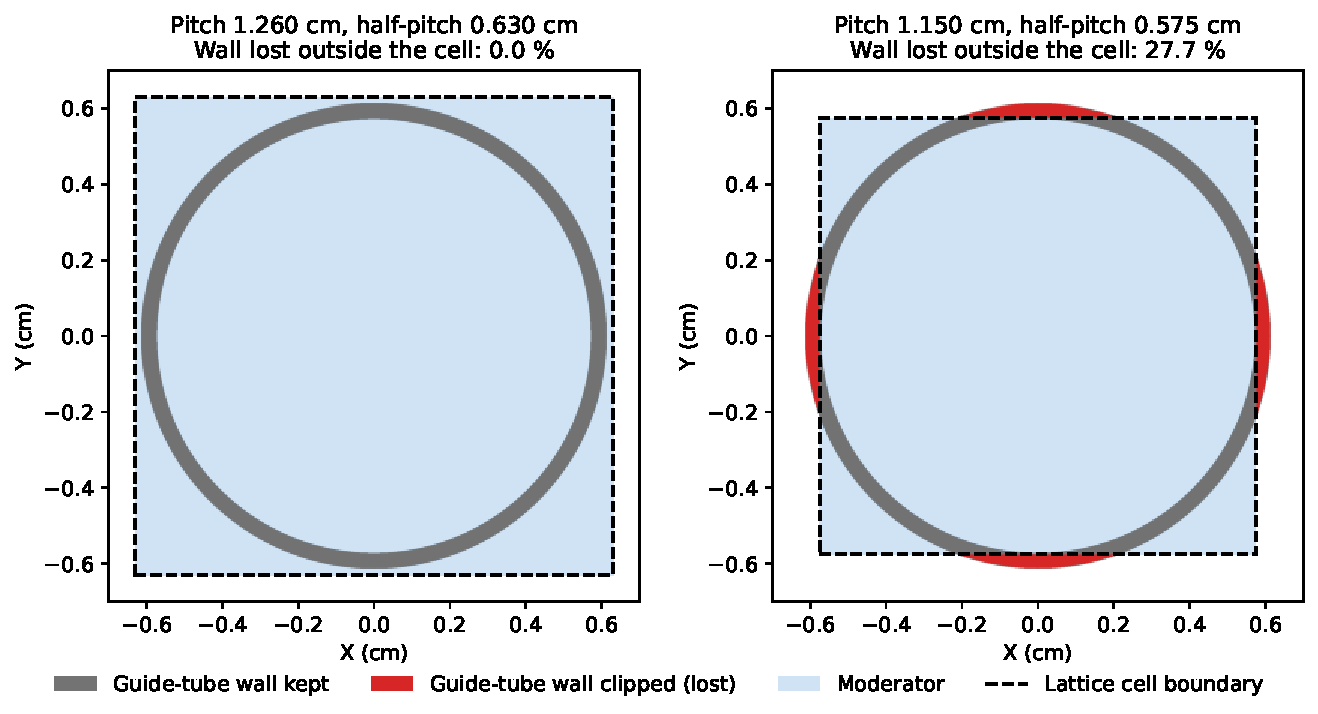
\includegraphics[width=0.75\linewidth]{images/th_gt_clip.pdf}
  \caption{Guide-tube wall and lattice cell at the reference pitch and at the lower pitch bound.}
  \label{fig:gt-clip}
\end{figure}


          \item The pitch is the design variable with the largest
                effect on the regulating-bank worth
                (Section~\ref{sec:res-c7-worth}).

          \item The pitch sets the moderator-to-fuel ratio, on which the
                moderator temperature coefficient
                depends~\cite{duderstadt_hamilton_1976}, and the coolant
                flow area and pressure drop~\cite{todreas_kazimi_2012}.
                The model has no thermal-hydraulic feedback, so it cannot
                itself show whether a given pitch is coolable. The pitch
                is therefore fixed at \SI{1.26}{cm}, the value of the
                operating $17\times17$ lattice, whose thermal-hydraulic
                performance over the enrichment range searched here is
                demonstrated by decades of service in commercial
                PWRs and documented in their
                safety analysis
                reports~\cite{epr_fsar_ch4,todreas_kazimi_2012}.
        \end{itemize}

  \item The two assembly enrichment zones collapse to one variable,
        since the core-level enrichment variation comes entirely from
        the ring multipliers of Section~\ref{sec:meth-zoning}. Its
        upper bound is \SI{13.913}{wt\%}, the value that holds the
        as-built peripheral ring at its own limit through
        Equation~\eqref{eq:leu-box}, so no proposed design can violate
        $g_\mathrm{enr}$.

  \item The vessel-fit constraint reserves a clearance
        $c_\mathrm{v} = \SI{7.08}{cm}$ for a core barrel and a
        downcomer: the \SI{5.08}{cm} stainless steel barrel of the
        reference specification and a \SI{2.0}{cm} downcomer, adopted
        as a minimum coolant return path. The clearance acts on the
        geometric constraint alone, since the campaign transport model
        keeps a vacuum boundary at the reflector surface
        (Section~\ref{sec:meth-barrel}).

  \item The reflector thickness is bounded by the radial budget that
        remains, Equation~\eqref{eq:refl-budget-c8}.
\end{enumerate}

\begin{equation}
t_\mathrm{refl}^{\max} = R_\mathrm{v} - c_\mathrm{v} - R_\mathrm{env}(p) - \delta
\label{eq:refl-budget-c8}
\end{equation}

\noindent where the symbols have the following meaning.

\begin{itemize}
  \item $t_\mathrm{refl}^{\max}$ is the largest reflector thickness that
        fits, \SI{5.669}{cm}, bounded in the design space at
        \SI{5.66}{cm} so that the box edge is strictly feasible.

  \item $R_\mathrm{v}$ is the vessel internal radius, \SI{90}{cm}.

  \item $c_\mathrm{v}$ is the reserved clearance, \SI{7.08}{cm}.

  \item $R_\mathrm{env}(p)$ is the circumscribed radius of the
        32-assembly fuel envelope at pitch $p$, \SI{77.231}{cm} at
        \SI{1.26}{cm}.

  \item $\delta$ is the lattice pad, \SI{0.02}{cm}.
\end{itemize}

Fixing the pitch has a cost that was known before the campaign, since
the designs of lowest peaking in Campaign 7 reach it with thick
reflectors that fit only at a narrow pitch and cannot be built at
\SI{1.26}{cm} (Section~\ref{sec:res-c5-c7}). Campaign 8 therefore
trades the minimum $F_{\Delta H}$ of Campaign 7 for a geometrically
valid lattice.

Both campaigns run the acquisition function of
Section~\ref{sec:meth-acq} at the two settings established in Campaign
6.

\begin{itemize}
  \item \textbf{Batch diversity distance:} $\delta_\mathrm{min} = 0.14$,
        the minimum normalised distance that separates any two designs
        of an infill batch. It acts on the selection of the batch and
        not on the constraints.

  \item \textbf{Feasibility margin coefficient:} $\kappa = 1.5$, the
        number of predictive standard deviations of the constraint
        surrogates that a candidate must hold in reserve to be ranked
        as margin-feasible.
\end{itemize}

Both are passed explicitly to the launcher after the Campaign 7
regression, in which the default values were used instead.

\subsection{Campaign 9 formulation}
\label{sec:meth-c9}

Campaigns 1 to 8 maximise the cycle length. In Campaign 8 every front
design has a cycle length well above the reported refuelling interval,
and the beginning-of-life excess reactivity that this cycle requires
can only be compensated by a deep insertion of the regulating banks
(Section~\ref{sec:res-c8-mission}). Campaign 9 therefore imposes the
required cycle length as a constraint and replaces it as an objective
by $c_\mathrm{max}$, the critical soluble boron concentration at the
reactivity maximum of the cycle. Minimising $c_\mathrm{max}$ directs the
search toward designs whose excess reactivity is held down by the
burnable absorbers rather than by the coolant, so the objective
measures how far each design stands from soluble-boron-free operation.

Campaign 9 takes the five-year refuelling interval reported for the
prototype~\cite{dinizcosta_2017} as the mission requirement, which
gives the floor of 1826 effective full power days used below.

\begin{equation}
\begin{aligned}
\min_{\mathbf{x}}\ &\big(F_{\Delta H}(\mathbf{x}),\ c_\mathrm{max}(\mathbf{x})\big) \\
\text{subject to}\ &\mathrm{EFPD}(\mathbf{x}) \ge 1826,\quad
F_{\Delta H}(\mathbf{x}) \le 1.65,\quad g_j(\mathbf{x}) \le 0
\end{aligned}
\label{eq:c9-problem}
\end{equation}

\noindent where the symbols have the following meaning.

\begin{itemize}
  \item $F_{\Delta H}$ is the radial peaking factor of the zoned core
        with all rods out at beginning of life, the objective of
        Campaign 8, dimensionless.

  \item $c_\mathrm{max}$ is the critical boron concentration at the
        operating maximum of the reactivity history, in ppm, defined in
        Equation~\eqref{eq:c9-cmax}.

  \item $\mathrm{EFPD}$ is the cycle length of
        Section~\ref{sec:objective_functions}.

  \item $1.65$ is the peaking constraint, reduced from the exploratory
        bound of 2.0 of Table~\ref{tab:constraints} to the Technical
        Specification limit of 1.65 of a licensed pressurised water
        reactor~\cite{robinson_gd10}.

  \item $g_j$ are the constraints $g_{k\min}$, $g_{k\max}$,
        $g_\mathrm{enr}$ and $g_\mathrm{geom}$ of
        Table~\ref{tab:constraints} with their Campaign 8 values, the
        controllability constraint $g_\mathrm{ctrl}$ at beginning of life, and the
        same constraint evaluated at the operating maximum,
        $g_\mathrm{ctrl,peak}$.
\end{itemize}

The critical concentration is computed inside the evaluator from
unrodded core solves at 1000, 2000 and, where the reactivity has not
yet changed sign, \SI{3000}{ppm}. The beginning-of-life concentration
$c_\mathrm{BOL}$ is the root of $\rho(c)$, found by interpolation
over the interval between the two solves across which $\rho(c)$
changes sign, or by extrapolation above the highest,
and the differential worth is its local slope at that root. The
concentration at the operating maximum adds the part of the gadolinium
hump that the boron has to hold, measured on the assembly depletion
history as a difference of reactivity.

\begin{equation}
\Delta\rho_\mathrm{hump} = \rho(k_\mathrm{peak}) - \rho(k_\mathrm{BOL}),
\qquad \rho(k) = 10^5\,\frac{k-1}{k}
\label{eq:c7-hump}
\end{equation}

\noindent where the symbols have the following meaning.

\begin{itemize}
  \item $\Delta\rho_\mathrm{hump}$ is the hump, in pcm. It is negative
        when beginning of life is the most reactive state of the design.

  \item $k_\mathrm{BOL}$ is the assembly $k_\infty$ at zero burnup,
        xenon-free, at \SI{1000}{ppm}, dimensionless.

  \item $k_\mathrm{peak}$ is the largest assembly $k_\infty$ over the
        operating points of the depletion history after beginning of
        life, dimensionless.

  \item $\rho$ is the reactivity, in pcm.
\end{itemize}

The concentration at the operating maximum then follows.

\begin{equation}
c_\mathrm{max} = c_\mathrm{BOL} + \frac{\max\!\big(L\,\Delta\rho_\mathrm{hump},\ 0\big)}{w_\mathrm{B}}
\label{eq:c9-cmax}
\end{equation}

\noindent where the symbols have the following meaning.

\begin{itemize}
  \item $c_\mathrm{BOL}$ is the critical boron concentration at
        beginning of life, in ppm.

  \item $\Delta\rho_\mathrm{hump}$ is the hump of
        Equation~\eqref{eq:c7-hump}, taken from the xenon-free assembly
        depletion history that the evaluator already computes, in pcm.
        A hump below \SI{400}{pcm} is set to zero. That floor is twice
        the seed-to-seed standard deviation of the hump at the
        Campaign 9 transport setting of $4\,000\times60$, which the
        seed-replicated study of
        Section~\ref{sec:res-c9-dep-check} measures at \SI{217}{pcm}, so
        a hump below it is not resolved by a single evaluation.

  \item $L$ is the ratio of the assembly to the core beginning-of-life
        eigenvalue of the same design, which carries the assembly hump
        to the core, dimensionless.

  \item $w_\mathrm{B}$ is the differential boron worth at the root, in
        pcm per ppm.
\end{itemize}

Two guards bound the objective where the measurement cannot reach it:

\begin{itemize}
  \item \textbf{A design that cannot be made critical without boron
        returns a negative root:} it is clamped at \SI{0}{ppm}, since a
        minimised objective would otherwise rank it best. Such designs
        are infeasible on $g_{k\min}$ in any case.

  \item \textbf{A root above the highest measured concentration is
        extrapolated:} it is clipped at \SI{6000}{ppm}, twice that
        concentration. Boron self-shielding makes the true root higher
        than the linear extrapolation predicts, so a clipped design
        keeps its place at the bottom of the archive.
\end{itemize}

\section{Leakage-corrected reactivity target}
\label{sec:meth-ktarget}

The cycle length of every design is obtained from the depletion of a
single fuel assembly under reflective boundaries
(Section~\ref{sec:objective_functions}), which carries no leakage,
while the core of 32 assemblies loses neutrons through its radial
boundary and has a lower eigenvalue at the same fuel composition. The
size of that gap across the design space is measured in
Section~\ref{sec:res-c5-c7}.

Placing the end of cycle where the assembly $k_\infty$ falls to one
would therefore overestimate every cycle length, since the core would
have become subcritical long before. Depleting the full core in every
evaluation would remove the error at a cost the optimisation loop
cannot afford, so the correction is applied to the end-of-cycle
criterion and not to the depletion model. The core is critical when
$k_\mathrm{eff}^\mathrm{core} = 1$, so if the ratio of the assembly to
the core eigenvalue stays constant during burnup, the core reaches
criticality when the assembly $k_\infty$ has fallen to that ratio. That
ratio is the leakage-corrected target of Section~\ref{sec:bg-k}.

\begin{equation}
k_\mathrm{target}(p, t_\mathrm{refl})
= \frac{k_\infty^\mathrm{assembly}}{k_\mathrm{eff}^\mathrm{core}}
\label{eq:ktarget}
\end{equation}

\noindent where the symbols have the following meaning.

\begin{itemize}
  \item $k_\mathrm{target}$ is the leakage-corrected end-of-cycle
        target entering Equation~\eqref{eq:eoc-k}, dimensionless.

  \item $k_\infty^\mathrm{assembly}$ is the infinite multiplication
        factor of the reflective single assembly, dimensionless.

  \item $k_\mathrm{eff}^\mathrm{core}$ is the effective multiplication
        factor of the two-dimensional 32-assembly core built with the
        same pitch and reflector thickness, dimensionless.

  \item $p$ is the pin pitch, in cm.

  \item $t_\mathrm{refl}$ is the reflector thickness, in cm.
\end{itemize}

One-group diffusion theory relates the two eigenvalues by
$k_\infty / k_\mathrm{eff} = 1 + M^2 B^2$, where $B^2$ is the geometric
buckling, in cm$^{-2}$, and $M^2$ the migration
area, in cm$^2$~\cite{duderstadt_hamilton_1976}. The two factors
depend on different quantities.

\begin{itemize}
  \item $B^2$ is determined by the size and the shape of the core
        alone. In this work the pitch determines the width of the
        32-assembly array and the reflector thickness the distance over
        which the flux decays outside it, so the two geometric design
        variables act here and the fuel does not.

  \item $M^2 = \tau + L^2$ is the mean square distance a neutron
        travels from birth to absorption, the Fermi age $\tau$ covering
        the slowing down and the diffusion area
        $L^2 = D / \Sigma_\mathrm{a}$ the thermal flight. This is where
        the composition enters. A higher enrichment or a gadolinia
        loading raises the absorption cross section
        $\Sigma_\mathrm{a}$, which shortens $L^2$ and with it $M^2$, so
        the leakage penalty falls.
\end{itemize}

Two consequences follow, and both were tested in
Section~\ref{sec:res-kt-burnup}. Over burnup the ratio is constant
within the Monte Carlo noise, no drift being resolved at two standard
deviations, so one evaluation serves the whole cycle. Across designs it
is not constant. The residual against the tabulated value is ordered by
enrichment and spans $+174$ to \SI{-329}{pcm}, which the same section
converts into a correction to the reported cycle length. The reference
composition carries no gadolinia because the criterion is applied at
end of cycle, where the gadolinium of every design has burnt out.

The ratio is therefore computed once, without depletion, at beginning
of life on a reference assembly of fresh fuel at \SI{4.05}{wt\%} in
the outer zone and \SI{4.55}{wt\%} in the inner zone:

\begin{itemize}
  \item at each pitch, one solve of the reflective assembly gives
        $k_\infty^\mathrm{assembly}$,

  \item at each pair of pitch and reflector thickness, one solve of the
        two-dimensional core gives $k_\mathrm{eff}^\mathrm{core}$.
\end{itemize}

The reference composition was fixed when the table was first
calibrated for Campaign 2, at the point where the target first had to
exist and before any campaign had returned a front to calibrate it on.
Its two enrichments sit inside commercial light water practice, below
the \SI{4.95}{wt\%} of the NuScale fuel design and the \SI{5}{wt\%}
that Section~\ref{subsec:comparison}
tabulates~\cite{nuscale_htp2_2017,iaea_smr_2024}, and it was not revised
once the campaigns began. Its error was measured a posteriori instead, in
Section~\ref{sec:res-kt-burnup}.

The $3\times7$ grid of Campaigns 2 to 7 thus required three assembly
solves and 21 core solves. Inside the loop the target is interpolated
bilinearly, so each evaluation needs only the depletion of its own
assembly, and the constancy of the ratio with burnup was tested once
the campaigns had run, on the Campaign 8 designs and on the Campaign 9
front (Section~\ref{sec:res-kt-burnup} and
Table~\ref{tab:c9-kt-burnup}).

\subsection{Axial leakage factor and the three-dimensional target}
\label{sec:meth-lax}

The leakage-corrected target of Equation~\eqref{eq:ktarget} corrects the
infinite-lattice depletion for the radial leakage of the
two-dimensional core. The transport model has no axial extent, so the
axial leakage of the finite core is absent from every cycle length of
Campaigns 1 to 7, and a dedicated study measured it before Campaign 8.

That study pairs each two-dimensional solve with a three-dimensional
one. The three-dimensional model extends the core to a finite active
height of \SI{120}{cm}, adds a \SI{15}{cm} slab of borated water above
and below the fuel as the axial reflector and places a vacuum boundary
beyond the slabs, the radial reflector spanning the full height. Its
materials and zoned enrichment map are those of the Campaign 6
evaluator, whose ring multipliers Campaigns 8 and 9 keep, so the axial
extent is the only difference between the two models and the ratio of
their eigenvalues isolates the axial leakage. Each paired
solve ran at \num{150000} particles and 200 batches with 80 inactive,
the raised inactive count allowing the axial source shape to converge,
in two seeds.

The axial leakage factor is the ratio of the two eigenvalues.

\begin{equation}
L_\mathrm{ax}(\mathbf{x}) = \frac{k_\mathrm{eff}^\mathrm{core}(\mathbf{x})}{k_\mathrm{eff}^\mathrm{core,3D}(\mathbf{x})}
\label{eq:lax-def}
\end{equation}

\noindent where the symbols have the following meaning.

\begin{itemize}
  \item $L_\mathrm{ax}$ is the axial leakage factor, dimensionless.

  \item $k_\mathrm{eff}^\mathrm{core}$ is the effective multiplication
        factor of the two-dimensional core of
        Equation~\eqref{eq:ktarget}, with the campaign radial reflector,
        dimensionless.

  \item $k_\mathrm{eff}^\mathrm{core,3D}$ is the effective
        multiplication factor of the same core at finite height with the
        axial reflectors, dimensionless.
\end{itemize}

The factor is measured in Section~\ref{sec:res-c5-c7}. Its value,
$L_\mathrm{ax} = \num{1.0289}$, is applied to every design with a
systematic uncertainty of $\pm\SI{80}{pcm}$.

Campaign 7 does not use it. That campaign carries one change of its
own, the measured controllability constraint, and under the one-change rule
of Section~\ref{sec:meth-campaigns} its target stays on the
two-dimensional table. From Campaign 8 the axial factor multiplies the
target, so that the end of cycle is defined on a finite-height core
from the start.

\begin{equation}
k_\mathrm{target}^\mathrm{3D}(t_\mathrm{refl}) = k_\mathrm{target}^\mathrm{2D}(t_\mathrm{refl}) \times L_\mathrm{ax}
\label{eq:ktarget-3d}
\end{equation}

\noindent where the symbols have the following meaning.

\begin{itemize}
  \item $k_\mathrm{target}^\mathrm{3D}$ is the target that the depleting
        assembly must retain at end of cycle for the finite core to be
        critical, dimensionless.

  \item $k_\mathrm{target}^\mathrm{2D}$ is the leakage-corrected target of
        Equation~\eqref{eq:ktarget} at the fixed pitch, dimensionless.

  \item $L_\mathrm{ax}$ is the axial factor, \num{1.0289}.

  \item $t_\mathrm{refl}$ is the reflector thickness, in cm.
\end{itemize}

The grid of Campaigns 2 to 7 cannot serve the fixed pitch. Its pitch
nodes are 1.15, 1.29 and \SI{1.43}{cm}, none of them \SI{1.26}{cm}, so
every evaluation would interpolate between two nodes and carry an
interpolation error in a variable that no longer varies. Its seven
reflector nodes are spread over 2.0 to \SI{19.5}{cm}, of which only two
fall inside the 2.0 to \SI{5.66}{cm} that the vessel-fit clearance
leaves to Campaign 8, so the resolution is lost exactly where the
search now works.

The calibration of Section~\ref{sec:meth-ktarget} was therefore
recomputed at the fixed pitch, where it depends on the reflector
thickness alone, with one assembly solve and seven core solves at
reflector nodes from 2.0 to \SI{5.66}{cm}. A weighted straight line
through those nodes replaces the raw values.

\begin{equation}
k_\mathrm{target}^\mathrm{2D}(t_\mathrm{refl}) = 1.054528 - 0.000516\, t_\mathrm{refl}
\label{eq:ktarget-c8-fit}
\end{equation}

The cycle lengths of Campaigns 8 and 9 therefore refer to a
finite-height core, and what the correction costs in cycle length is
reported in Section~\ref{sec:res-c8}.


\section{Radial zoning and enrichment bounds}
\label{sec:meth-zoning}

From Campaign 6 the beginning-of-life core map is zoned radially inside
the evaluator, so the peaking objective and the peaking constraint act
on the zoned core rather than on a uniform loading.

The 32-assembly map is partitioned into three concentric rings by the
Euclidean distance of each assembly position from the centre of the
map, measured in lattice units.

\begin{enumerate}
  \item Ring C, the centre, 4 assemblies at a distance below 1.0.
  \item Ring M, the middle, 12 assemblies at a distance from 1.0 to
        2.3.
  \item Ring P, the periphery, 16 assemblies at a distance of 2.3 or
        above.
\end{enumerate}

Figure~\ref{fig:zoning-rings} shows the three rings on the core map.

\begin{figure}[htbp]
  \centering
  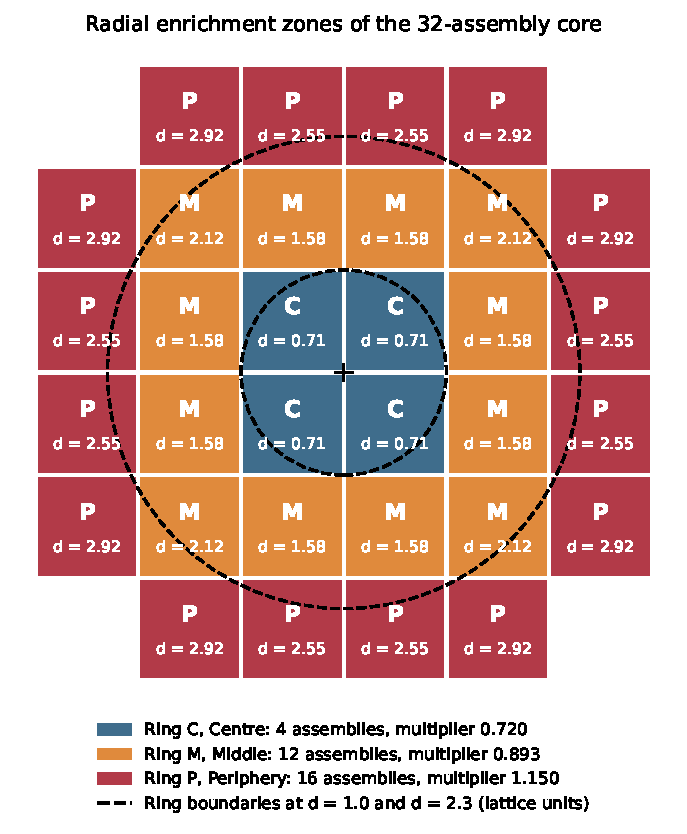
\includegraphics[width=0.75\linewidth]{images/th_zoning_rings.pdf}
  \caption{Radial enrichment rings of the 32-assembly core.}
  \label{fig:zoning-rings}
\end{figure}

The enrichment of each ring is the corresponding design enrichment
scaled by a fixed ring multiplier.

\begin{equation}
e_r \;=\; m_r \, e, \qquad r \in \{C, M, P\}
\label{eq:zoning}
\end{equation}

\noindent where the symbols have the following meaning.

\begin{itemize}
  \item $e_r$ is the as-loaded enrichment of ring $r$, in
        wt\%~$^{235}$U.

  \item $e$ is the design enrichment assigned to that ring, in
        wt\%~$^{235}$U.

  \item $m_r$ is the multiplier of ring $r$, dimensionless, equal to
        $m_C = 0.720$ for the centre, $m_M = 0.893$ for the middle
        ring and $m_P = 1.150$ for the periphery.
\end{itemize}

Only $m_C$ and $m_P$ are set. The middle multiplier is solved from the
fissile balance, which holds the assembly-weighted mean multiplier of
the core at one.

\begin{equation}
n_C\,m_C + n_M\,m_M + n_P\,m_P = n_C + n_M + n_P
\label{eq:zoning-balance}
\end{equation}

\noindent where $n_C$, $n_M$ and $n_P$ are the assembly counts of the
three rings, equal to 4, 12 and 16, dimensionless. With $m_C = 0.720$
and $m_P = 1.150$ the balance returns $m_M = 0.893$, so the zoned core
and an unzoned core built from the same enrichment variables carry the
same fissile inventory.

\subsection{How the design enrichments enter the rings}
\label{sec:meth-zoning-map}

The zoning does not assign one design enrichment to one ring. Through
Campaign 7 every assembly of the core keeps the two-zone
intra-assembly structure of Table~\ref{tab:model-geometry}, illustrated in
Figure~\ref{fig:model-geometry}(a), namely the centred $9\times9$ block
of 72 rods at $e_\mathrm{in}$ and the surrounding 192 rods at
$e_\mathrm{out}$. What the ring multiplier does is scale \emph{both}
intra-assembly enrichments of every assembly in that ring by the same
factor. From Campaign 8 the two zones collapse to the single enrichment
variable of Section~\ref{sec:meth-c8-space}, and the multiplier scales
that one value.

\begin{equation}
e_\mathrm{in}^{\,r} = m_r \, e_\mathrm{in},
\qquad
e_\mathrm{out}^{\,r} = m_r \, e_\mathrm{out}
\label{eq:zoning-pair}
\end{equation}

\noindent where the symbols have the following meaning.

\begin{itemize}
  \item $e_\mathrm{in}^{\,r}$ and $e_\mathrm{out}^{\,r}$ are the
        as-loaded inner-zone and outer-zone enrichments of an assembly
        in ring $r$, in wt\%~$^{235}$U.

  \item $e_\mathrm{in}$ and $e_\mathrm{out}$ are the two enrichment
        design variables, in wt\%~$^{235}$U.

  \item $m_r$ is the multiplier of ring $r$, dimensionless.
\end{itemize}

Three consequences follow, and all three are properties of the
implementation rather than modelling choices imposed a posteriori.

\begin{enumerate}
  \item Zoning is an enrichment redistribution only. Pitch, reflector
        thickness, gadolinia weight fraction and gadolinia rod count
        are copied to every ring unchanged, so the three ring
        assemblies are built by the same builders with the same pin
        layout as the base assembly.

  \item The gadolinia rods of each ring take their \ce{^{235}U}
        enrichment from that ring, reduced by 5 per cent, relative, per
        wt\% of \ce{Gd2O3}, with a lower limit of \SI{0.2}{wt\%}
        (Table~\ref{tab:in-materials}), following the practice for
        low-concentration gadolinia fuel~\cite{mildrum_segovia_2001}.
        The reduction lowers the fissile
        content of the urania--gadolinia rods, whose thermal conductivity
        is lower than that of \ce{UO2}~\cite{mildrum_segovia_2001}. At
        \SI{8}{wt\%} of \ce{Gd2O3}, for example, the factor is 0.60, so
        the gadolinia rods of a peripheral ring at \SI{11.5}{wt\%} carry
        \SI{6.9}{wt\%}.

  \item The zoning is applied on core solves only. The beginning-of-life
        core solve of Section~\ref{sec:meth-core-objective} and the two
        rodded solves of Section~\ref{sec:meth-ctrl} are built from the
        zoned map, while the depletion of
        Section~\ref{sec:objective_functions} runs on the assembly
        loaded at the design enrichments themselves, with no multiplier
        applied, that is $m = 1$ in
        Equation~\eqref{eq:zoning-pair}. That assembly is none of the
        three rings. It carries the core-average fissile loading, since
        the balance of Equation~\eqref{eq:zoning-balance} holds the
        assembly-weighted mean multiplier at one, and the reflective
        boundary of the depletion model replicates it into an infinite
        lattice of identical assemblies. The burnup history obtained is
        therefore the history of a core of 32 such replicas, whose
        fissile inventory equals that of the zoned core.
\end{enumerate}

%% labels of the material summarised in the zoning section, kept so that the
%% cross-references of the other chapters still resolve
\label{sec:meth-zoning-balance}

%% labels of the material reported in the results, kept so that the
%% cross-references of the other chapters still resolve
\label{sec:meth-zoning-study}\label{tab:zoning-transfer}\label{tab:zoning-grid}

\subsection{The enrichment search box}
\label{sec:meth-zoning-box}

Because the periphery carries the largest multiplier, the
low-enriched-uranium enrichment limit binds through the as-loaded peripheral ring
and not through the design variable directly. From Campaign 6 the
enrichment constraint is therefore written on the zoned map.

\begin{equation}
g_\mathrm{enr} \;=\; \max_r \left( m_r\, e \right) - 19.75 \;\le\; 0
\quad\Longrightarrow\quad
e \;\le\; \frac{19.75}{m_P} \;=\; 17.174
\label{eq:leu-box}
\end{equation}

\noindent where the symbols have the following meaning.

\begin{itemize}
  \item $g_\mathrm{enr}$ is the enrichment-limit constraint of
        Table~\ref{tab:constraints}, in wt\%~$^{235}$U, redefined on
        the zoned map from Campaign 6.

  \item $19.75$ is the low-enriched-uranium limit, in
        wt\%~$^{235}$U.

  \item $m_P$ is the peripheral multiplier, dimensionless, equal to
        1.150.

  \item $17.174$ is the resulting upper bound of both enrichment
        design variables in Campaign 6, in wt\%~$^{235}$U.
\end{itemize}

The box bound and the constraint are consistent by construction, so no
design of experiments point can violate the limit after zoning. This
removes the wasted samples observed under the earlier formulation, and
it is also what bounds $m_P$ from above.

The value of $m_P$ is the only decision of this section that is not
fixed by a measurement. A larger multiplier lowers the radial peaking
factor further, but it lowers the upper enrichment bound of
Equation~\eqref{eq:leu-box} in the same proportion, and the enrichment
limit was already active in Campaign 5. Campaign 6 therefore adopts
$m_P = 1.150$, keeping the wider enrichment range at the cost of that
peaking reduction, and a later campaign can raise $m_P$ if the
enrichment bound is no longer active. The trial on which the value was
set is reported in Section~\ref{sec:res-c5-c7}.

The zoning is the only change of Campaign 6 that acts on the
beginning-of-life power distribution, so the peaking reduction of
Campaign 6 is attributed to it (Section~\ref{sec:res-c6-compare}).
\section{Burnup limits in the simulations}
\label{sec:meth-atf}

Two assembly-average burnup limits act on the depletion of
Section~\ref{sec:bg-depletion}:

\begin{itemize}
  \item the discharge-burnup limit $B_\mathrm{burnup}$, which decides
        whether a design is acceptable and, through
        Equation~\eqref{eq:efpd}, truncates its reported cycle length,

  \item the depletion horizon $B_\mathrm{max}$, the burnup at which the
        depletion calculation is stopped.
\end{itemize}

The limit is $B_\mathrm{burnup} = \SI{55}{MWd/kgHM}$, the
assembly-average exposure limit of uranium dioxide in zirconium
cladding, set by cladding oxidation~\cite{song_sanchez_2026,alam_2019_hotchannel}.
The corresponding rod-average limit is \SI{62}{MWd/kgHM}. The limit is
applied at candidate selection to
the archived end-of-cycle burnups, so it needs no new transport
calculation. It removes designs from the fronts of Campaigns 6 and 8
and leaves those of Campaigns 7 and 9 unchanged, as reported with each
campaign.

The horizon has changed with the campaigns. Campaign 1 stopped the
depletion at \SI{35.5}{MWd/kgHM}, Campaign 2 raised it to
\SI{100}{MWd/kgHM} to test whether the censoring was an artefact of the
stopping value, and Campaigns 3 to 5 stopped at the \SI{75}{MWd/kgHM}
then adopted as the discharge limit
(Section~\ref{sec:res-c5-c7}). From Campaign 6 onwards the horizon is
$B_\mathrm{max} = \SI{100}{MWd/kgHM}$, well above the limit, so that
designs reach the end-of-cycle target before the depletion stops. Right-censoring then becomes rare, and
the objective surrogate is not trained on censored cycle lengths. Its prediction is
clipped at the horizon by Equation~\eqref{eq:efpd-clip}.

\section{Moderator temperature coefficient and the MTC boron limit}
\label{sec:meth-mtc}

The reference concentration of Section~\ref{sec:meth-boron} is held at
\SI{1000}{ppm} throughout the optimisation, so the campaigns do not test
whether a candidate can be held critical by soluble boron at an
acceptable concentration. That concentration has an upper limit. A rise
in moderator temperature lowers the moderator density, and with it the
boron number density in the core, which inserts positive reactivity.
This contribution grows with the boron concentration, and above a
certain concentration the moderator temperature coefficient becomes
positive. A positive coefficient removes the negative temperature
feedback that stabilises the core against a power excursion, and it is
not acceptable at power. The concentration at which the coefficient is
zero is therefore the upper limit of the soluble boron, called here the
MTC boron limit, and it depends on the lattice.

\subsection{Definition and evaluation}
\label{sec:meth-mtc-def}

The coefficient is evaluated as a two-point difference at constant
pressure, with the moderator density taken consistently with the
temperature from the IAPWS-IF97 formulation~\cite{wagner_iapws_if97_2000}.

\begin{equation}
\alpha_\mathrm{M}(c) = \frac{\rho\!\left(T + \Delta T,\ c\right)
- \rho\!\left(T,\ c\right)}{\Delta T}
\label{eq:mtc}
\end{equation}

\noindent where the symbols have the following meaning.

\begin{itemize}
  \item $\alpha_\mathrm{M}$ is the moderator temperature coefficient, in
        pcm per K.
  \item $\rho$ is the core reactivity at the stated moderator temperature
        and soluble boron concentration, in pcm.
  \item $T$ is the moderator temperature, in K, with the density set from
        the steam tables at the operating pressure.
  \item $\Delta T$ is the temperature perturbation, in K.
  \item $c$ is the soluble boron concentration, in ppm.
\end{itemize}

The zero-coefficient concentration $c_\mathrm{MTC}$ is the root of
Equation~\eqref{eq:mtc} in concentration. It is obtained by a weighted
straight-line fit of the coefficient against concentration over the
three scan points nearest the sign change, with the uncertainty
propagated from the fit covariance and inflated by $\sqrt{\chi^2/\nu}$
where that exceeds unity, so that it reflects a curvature of the
coefficient in boron.

\begin{equation}
\alpha_\mathrm{M}\!\left(c_\mathrm{MTC}\right) = 0
\label{eq:ceiling}
\end{equation}

\noindent where $c_\mathrm{MTC}$ is the MTC boron limit, in ppm.

A design is acceptable on this criterion when its critical concentration
at beginning of life, the root of the measured reactivity $\rho(c)$, or
its cycle maximum of Equation~\eqref{eq:c9-cmax} where a positive hump
is resolved, does not exceed $c_\mathrm{MTC}$.

The limit is evaluated outside the optimisation loop, recorded in the
archive as $g_\mathrm{boron}$ and never imposed as a constraint. Each
scan solves the zoned core at two moderator temperatures and four boron
concentrations, with two seeds per point at $100\,000$ particles and 170
batches. It was run on C8-47 at both pressures below, and on eight
Campaign 9 lattices at \SI{12.8}{MPa}, five of them also at
\SI{15.5}{MPa}.

The two best-ranked designs, C8-47 and C9-47, are scanned at each pressure both on
a two-dimensional core and on the three-dimensional core model of
Section~\ref{sec:res-c8-3d}, with the control rods fully withdrawn above the active core, so the
limit and the three-dimensional confirmation rest on the same geometry.
The pair of scans separates the axial leakage contribution to the limit
from the lattice contribution. The other seven Campaign 9 designs are
scanned on the three-dimensional core model only, because the axial
leakage contribution to the limit is measured on the two best-ranked
designs and is not the quantity that separates one design from another.

Two temperature intervals were scanned, each centred on the average
coolant temperature of a reference plant:

\begin{itemize}
  \item 570 to \SI{590}{K} at \SI{15.5}{MPa}, centred on the moderator
        temperature of \SI{580}{K} of Table~\ref{tab:model-operating},
        with moderator densities of 0.733 and \SI{0.688}{g/cm^3}
        and saturation at \SI{617.9}{K}.
        These are the primary pressure and the average coolant
        temperature of a large pressurised water
        reactor~\cite{todreas_kazimi_2012,epr_fsar_ch4},

  \item 547 to \SI{567}{K} at \SI{12.8}{MPa}, centred on \SI{557}{K},
        with moderator densities of 0.771 and \SI{0.734}{g/cm^3}
        and saturation at \SI{602.8}{K}.
        These are the system pressure, \SI{12.76}{MPa}, and the core
        average temperature, \SI{557}{K}, of the NuScale
        module~\cite{nuscale_htp2_2017}.
\end{itemize}

The limit depends on the pressure through the moderator density. No
open source gives the primary conditions of LABGENE or of any naval
propulsion reactor, so the two intervals are reference points and carry
no claim about the prototype.

The two-dimensional core omits the axial component of the moderator
feedback. When the moderator heats and expands, the axial leakage grows
and adds negative reactivity, so a limit evaluated in two dimensions
is too low. The omitted term is the difference between the three- and
the two-dimensional coefficients at the same state.

\begin{equation}
\alpha_\mathrm{ax} = \alpha_\mathrm{M}^\mathrm{3D} - \alpha_\mathrm{M}^\mathrm{2D}
\label{eq:axial-feedback}
\end{equation}

\noindent where $\alpha_\mathrm{ax}$ is the axial leakage contribution
and $\alpha_\mathrm{M}^\mathrm{3D}$ and $\alpha_\mathrm{M}^\mathrm{2D}$
are the moderator temperature coefficients in three and in two
dimensions, all in pcm per K. The two-dimensional limit is therefore
reported as a conservative bound and the three-dimensional limit as
the physical result.


%% labels of the material summarised in the definition above, kept so that the
%% cross-references of the other chapters still resolve
\label{sec:meth-mtc-checks}

%% labels of the material reported in the results, kept so that the
%% cross-references of the other chapters still resolve


\section{Transport fidelity and seeding}
\label{sec:meth-fidelity}

Every quantity returned by the evaluator is a Monte Carlo estimate,
and every one of them carries a statistical uncertainty set by the
number of neutron histories. The eigenvalue and the cycle length carry
that uncertainty alone: they are unbiased, and their error is
symmetric about the true value
(Section~\ref{sec:bg-mc-stats})~\cite{lux_koblinger_1991}. The peaking
factor $F_{\Delta H}$ carries a positive bias on top of it, for the
reason given in Section~\ref{sec:meth-fdh}. Both the bias and the
variance fall as the number of active histories grows, and the cost of
the solve grows with them.

Two settings of the transport solve therefore control the quality of
every result of this work.

\begin{itemize}
  \item \textbf{Fidelity:} the number of particles per batch and the
        number of active and inactive batches. It sets the relative
        standard error of every tally and the bias of the peaking
        estimator.

  \item \textbf{Seed policy:} the rule that assigns the initial seed of
        the pseudo-random number generator. It decides whether two
        evaluations are driven by the same random-number sequence, and
        with it whether their statistical noise is correlated.
\end{itemize}

The need to control both was established in Campaign 2
(Section~\ref{sec:res-c1c2}). At the fidelity of that campaign,
$4\,000\times60$ with one shared seed, the bias of the stored peaking
values was larger than the spread of the front they ranked, and
re-solving the candidates at high fidelity re-ordered them.

\subsection{Fidelity study}
\label{sec:meth-fid-ladder}

The fidelity of the high-fidelity search was chosen from a
seed-replicated study of the assembly estimator, in which the same
designs are repeated at $4\,000$, $16\,000$, $64\,000$ and
$256\,000$ particles with independent seeds, so that the
seed-to-seed standard deviation measures the noise and the difference
to the highest setting measures the bias. The study is reported in
Section~\ref{sec:res-c1c2}, and its outcome is the
$16\,000\times120$ setting adopted for the high-fidelity search of
Campaigns 3 and 5, which removes most of the bias for nine times the
number of active histories: \num{16000} particles over 90 active
batches is \num{1440000} histories, against \num{160000} for
\num{4000} particles over 40 active batches.

A second study measures the core estimator. The study of
Table~\ref{tab:fid-ladder} covers the assembly estimator, which is the
peaking objective of Campaigns 3 and 5 only, while from Campaign 4 the
objective is the core estimator at $100\,000\times170$ (60 inactive),
whose maximum is taken over the pins of the zoned 32-assembly core. Its
bias is taken against the extrapolation of each design to an infinite
number of histories.

\begin{equation}
F_{\Delta H}(N) = F_\infty + \frac{a}{\sqrt{N}}
\label{eq:fdh-extrap}
\end{equation}

\noindent where $F_{\Delta H}(N)$ is the mean over the seeds of the core
peaking factor at $N$ active histories, the particles per batch
multiplied by the 110 active batches, $F_\infty$ is the extrapolated
value and $a$ the fitted bias coefficient, all dimensionless. The
extrapolation assumes that the bias falls as $1/\sqrt{N}$. The study
that applies it is reported in Section~\ref{sec:res-c9-peaking}.

\subsection{Transport settings per campaign}
\label{sec:meth-fid-settings}

Table~\ref{tab:fidelity} lists the transport settings of every campaign
and evaluation stage. A campaign row gives the settings of the assembly
depletion run in every evaluation of that campaign. The other rows are
evaluation stages, that is, transport calculations run in addition to
the assembly depletion: the core solves inside each evaluation from
Campaign 4, and the two stages at higher fidelity with which the
finalists of Campaigns 2 and 3 were ranked.
The settings are stored in each campaign checkpoint and cannot change
during a campaign.

\begin{table}[htbp]
  \centering
  \begin{threeparttable}
  \caption{Transport settings per campaign and per evaluation stage.}
  \label{tab:fidelity}
  \small
  \begin{tabularx}{\textwidth}{@{}>{\raggedright\arraybackslash}p{0.21\textwidth}c>{\raggedright\arraybackslash}p{0.17\textwidth}>{\raggedright\arraybackslash}X@{}}
    \toprule
    Stage & Particles $\times$ batches\tnote{a} & Seed policy & Role \\
    \midrule
    Campaign 1     & $4\,000\times60$ (20)    & shared              & verification \\
    Campaign 2     & $4\,000\times60$ (20)    & shared              & low-fidelity search \\
    Campaign 3     & $16\,000\times120$ (30)  & per-design          & high-fidelity search \\
    C4 core solve  & $100\,000\times170$ (60) & per-design, salted  & core solve: $F_{\Delta H}$ \\
    Campaign 5     & $16\,000\times120$ (30)  & per-design          & high-fidelity search \\
    C5 confirmation & $200\,000\times260$ (80) & replicated, 8 seeds & confirmation of one design \\
    Campaign 6     & $4\,000\times60$ (20)    & per-design          & low-fidelity search \\
    C6 core solve  & $100\,000\times170$ (60) & per-design, salted  & core solve: $F_{\Delta H}$, $k$ window \\
    Campaign 7     & $4\,000\times60$ (20)    & per-design          & low-fidelity search \\
    C7 core solves & $100\,000\times170$ (60) & per-design, salted  & core solves: $F_{\Delta H}$, $k$ window, one rodded solve \\
    Campaign 8     & $4\,000\times60$ (20)    & per-design          & low-fidelity search \\
    C8 core solves & $100\,000\times170$ (60) & per-design, salted  & core solves: $F_{\Delta H}$, $k$ window, two rodded solves \\
    Campaign 9     & $4\,000\times60$ (20)    & per-design          & low-fidelity search \\
    C9 core solves & $100\,000\times170$ (60) & per-design, salted  & core solves: as C8, and unrodded at 2000 and 3000\,ppm for $c_\mathrm{max}$ \\
    Preselection   & $64\,000\times120$ (30)  & replicated          & selection, first stage \\
    Confirmation   & $256\,000\times120$ (30) & replicated, 8 seeds & selection, second stage \\
    \bottomrule
  \end{tabularx}
  \begin{tablenotes}[flushleft]\footnotesize
    \item[a] Inactive batches in parentheses.
  \end{tablenotes}
  \end{threeparttable}
\end{table}

From Campaign 6 the assembly depletion returns to $4\,000\times60$,
the setting of Campaigns 1 and 2, after the $16\,000\times120$ of
Campaigns 3 and 5. The change is part of a two-tier fidelity strategy. The search runs at low fidelity,
where it needs many evaluations and the cycle length can carry a known
bias, while the core solves inside each evaluation, which evaluate
$F_{\Delta H}$, the reactivity window and the controllability constraints, stay at
$100\,000\times170$. Feasibility and peaking are therefore computed at
full fidelity, and only the cycle length carries the low-fidelity bias,
so the cycle lengths of Campaigns 6 to 9 are not comparable with those
of Campaigns 3 to 5 without a measured inter-fidelity shift, which
Section~\ref{sec:res-c9-dep-check} reports. The fidelity is held
constant across all blocks of a campaign, because a surrogate trained
on a mixed-fidelity archive carries a bias that changes with the
evaluation date and cannot be corrected a posteriori. The second tier
is the three-dimensional confirmation of the Campaign 8 candidates of
Section~\ref{sec:res-c8-limits}, and every Campaign 6 and Campaign 7
cycle length remains a low-fidelity value.

\subsection{Seed policy}
\label{sec:meth-fid-seed}

OpenMC initialises its pseudo-random number generator with the same
default seed in every run unless another seed is set. With that
default, every design is computed on the same random-number sequence.
Two similar problems driven by one sequence consume the same random
numbers at the same points of each history, so the source sites and
the interaction outcomes they sample coincide until the two models
differ. Their tally errors then share a common component and the noise
of different designs is positively correlated, which is the mechanism
of correlated sampling~\cite{lux_koblinger_1991}.

The coupling is partial
here, because two designs differ in geometry and composition and their
histories diverge as soon as that difference changes a sampled
interaction. Campaigns 1 and 2 ran on that default seed, so every
design of both campaigns shared one sequence. The effect was detected
in Campaign 2, where re-solving the finalists at high fidelity with
independent seeds did not preserve their ranking
(Section~\ref{sec:res-c1c2}).

From Campaign 3 each design receives its own seed, a CRC32 hash of its
design vector. Each core solve adds a fixed string to the hash, the
salt, so that the assembly and core solves of one design also run on
different sequences. The policy has two properties.

\begin{itemize}
  \item \textbf{Reproducibility:} the seed depends only on the design,
        so repeating an evaluation returns the same result.

  \item \textbf{Independent noise:} the noise of two designs is
        uncorrelated, which is the independent and identically
        distributed noise assumed by the white-noise term of the
        Gaussian-process kernel of Section~\ref{sec:bg-gp}.
\end{itemize}

%% labels of the removed section, kept so that the cross-references still resolve
\label{sec:meth-stats}\label{eq:noise-margin-set}

\section{Surrogate-assisted active-learning loop}
\label{sec:meth-loop}

The loop is described in Section~\ref{sec:bg-al} and
Figure~\ref{fig:bg-al}. One iteration has four steps.

\begin{enumerate}
  \item A Latin-hypercube design of experiments.

  \item Gaussian-process surrogates of the objectives and the
        constraints (Section~\ref{sec:bg-gp}).

  \item An NSGA-II search on the surrogates
        (Section~\ref{sec:bg-nsga2}).

  \item An infill batch evaluated with OpenMC.
\end{enumerate}

This section fixes what Chapter~\ref{ch:background} leaves open.

\begin{enumerate}
  \item The stopping rule.

  \item The settings with which the loop was run.

  \item The acquisition function, with the three revisions that
        Campaign 6 made necessary.
\end{enumerate}

Figure~\ref{fig:meth-loop-flow} summarises one iteration as
implemented.

\begin{figure}[htbp]
  \centering
  \resizebox{\textwidth}{!}{%
  \begin{tikzpicture}[
      box/.style={draw, rounded corners=2pt, align=center, font=\small,
                  text width=2.35cm, minimum height=1.35cm, fill=blue!6},
      outbox/.style={box, fill=green!10},
      arr/.style={-{Stealth[length=2.2mm]}, thick},
      node distance=0.45cm]
    \node[box] (a) {Archive of OpenMC evaluations};
    \node[box, right=of a] (b) {Fit one GP per objective and constraint};
    \node[box, right=of b] (c) {NSGA-II on the surrogates, $300\times400$};
    \node[box, right=of c] (d) {Rank-1 candidate set};
    \node[box, right=of d] (e) {Acquisition: infill batch of six};
    \node[box, right=of e] (f) {OpenMC evaluation and checkpoint};
    \node[outbox, right=0.9cm of f] (g) {Pareto front of the archive};
    \draw[arr] (a) -- (b);
    \draw[arr] (b) -- (c);
    \draw[arr] (c) -- (d);
    \draw[arr] (d) -- (e);
    \draw[arr] (e) -- (f);
    \draw[arr] (f) -- node[above, font=\footnotesize, align=center] {rule\\met} (g);
    \draw[arr] (f.south) -- ++(0,-0.55) -| node[pos=0.25, below, font=\footnotesize]
      {Stopping rule not met: next iteration} (a.south);
  \end{tikzpicture}}
  \caption{One iteration of the surrogate-assisted loop.}
  \label{fig:meth-loop-flow}
\end{figure}

\subsection{Stopping rule}
\label{sec:meth-loop-stop}

The loop stops when two conditions hold together. The first uses the
relative gain of the hypervolume of Section~\ref{sec:bg-hv} in each
iteration.

\begin{equation}
\Delta_t = \frac{H_t - H_{t-1}}{H_{t-1}}
\label{eq:hv-stop}
\end{equation}

\noindent where $\Delta_t$ is the relative gain of iteration $t$,
dimensionless, and $H_t$ and $H_{t-1}$ are the hypervolumes of the
archive after iterations $t$ and $t-1$, Equation~\eqref{eq:hv}, against
the fixed reference point. The condition is that the gain stays below
one per cent in each of the last three iterations:

\begin{equation}
\Delta_{T-2} < 0.01, \qquad \Delta_{T-1} < 0.01, \qquad \Delta_{T} < 0.01
\label{eq:hv-stop-cond}
\end{equation}

\noindent where $T$ is the last iteration completed.

The second condition is that no censored design remains on the Pareto
front, so that the front is fully resolved. A three-iteration window is
used because the gains are not monotonic.

The rule is necessary and not sufficient, since it can fire while the
acquisition selects near-duplicate or infeasible designs
(Section~\ref{sec:res-c6-margin}). Two health indicators are therefore recorded at every iteration and
checked before the rule is accepted:

\begin{itemize}
  \item the number of candidates that pass the feasibility margin of
        Equation~\eqref{eq:feas-margin}, which shows whether the
        constraint surrogate is still changing,

  \item the depth of the separation relaxation of
        Section~\ref{sec:meth-acq}, which shows whether the surrogate
        front still contains new designs.
\end{itemize}

Campaigns 3 and 6 met the rule. Campaigns 8 and 9 were stopped at
their budget of 60 evaluations, one iteration short of the window, and
their fronts are reported as the best available at that budget
(Sections~\ref{sec:res-c8-limits} and~\ref{sec:res-c9-convergence}).

\subsection{Surrogate and loop settings}
\label{sec:meth-loop-settings}

The inputs and outputs of every Gaussian process are standardised, so
that one dimensionless length-scale per variable of
Equation~\eqref{eq:kernel-r} is meaningful.

\begin{equation}
z_d = \frac{x_d - \bar{x}_d}{s_d}
\label{eq:standardise}
\end{equation}

\noindent where $z_d$ is the standardised value of variable $d$,
dimensionless, and $\bar{x}_d$ and $s_d$ are the mean and the standard
deviation of that variable over the archive, in its native unit. The
outputs are standardised in the same way.

One independent Gaussian process with the kernel of
Equation~\eqref{eq:kernel} is fitted to each output, the two objectives
and every constraint that is not computed analytically. Its
hyperparameters are refitted on the whole archive by maximising the log
marginal likelihood~\cite{rasmussen_gp_2006}. The refit is performed
once per iteration of the active-learning loop, that is once the
OpenMC evaluations of an infill batch have entered the archive. The
generations of the NSGA-II search run on surrogates whose
hyperparameters are held fixed and are not refitted.

\begin{equation}
\log p(\mathbf{y} \mid \boldsymbol{\theta})
= -\tfrac{1}{2}\,\mathbf{y}^{\mathsf T}
\left( \mathbf{K} + \sigma_n^{2}\mathbf{I} \right)^{-1} \mathbf{y}
- \tfrac{1}{2} \log \left| \mathbf{K} + \sigma_n^{2}\mathbf{I} \right|
- \tfrac{n}{2} \log 2\pi
\label{eq:gp-lml}
\end{equation}

\noindent where $\boldsymbol{\theta} = (\ell_1, \dots, \ell_D,
\sigma_f, \sigma_n)$ is the vector of hyperparameters and the other
symbols are those of Equations~\eqref{eq:kernel} to~\eqref{eq:gp-var}.
The maximisation is restarted from four random starting points to avoid
a local maximum. The first term rewards the fit to the archive and the
second penalises model complexity, so the fitted length-scales do not
simply interpolate the noise.

Table~\ref{tab:loop-settings} gives the loop settings of Campaigns 3
to 9. Campaign 3 is the first campaign in which per-design seeding made
the archive statistically consistent.

\begin{table}[htbp]
  \centering
  \small
  \caption{Loop settings per campaign.}
  \label{tab:loop-settings}
  \begin{tabular}{@{}lccccl@{}}
    \toprule
    Campaign & Initial designs & Batch & Iterations & Total & End \\
    \midrule
    C3 & 36 & 6 & 6  & 72  & stopping rule met \\
    C4 & 36 & 6 & 3  & 54  & -- \\
    C5 & 42 & 6 & 3  & 60  & -- \\
    C6 & 42 & 6 & 12 & 114 & stopping rule met \\
    C7 & 42 & 6 & 3  & 60  & -- \\
    C8 & 36 & 6 & 4  & 60  & budget, best available \\
    C9 & 24 & 6 & 6  & 60  & budget, best available \\
    \bottomrule
  \end{tabular}
\end{table}

\subsection{Acquisition function}
\label{sec:meth-acq}

The infill batch is selected from the rank-1 set of the final NSGA-II
population on the surrogates. The base criterion, whose steps are
listed in Section~\ref{sec:bg-al}, ranks the candidates by their
aggregated predictive uncertainty.

\begin{equation}
a_i \;=\; \sum_{m=1}^{2} \frac{\sigma_{im}}{\max_{l}\,\sigma_{lm}}
\label{eq:acq-score}
\end{equation}

\noindent where $a_i$ is the acquisition score of candidate $i$,
dimensionless, and $\sigma_{im}$ is the posterior standard deviation of
objective $m$ at candidate $i$ from Equation~\eqref{eq:gp-var}. The
index $l$ runs over the same rank-1 candidate set as $i$, so
$\max_l \sigma_{lm}$ is the largest posterior standard deviation of
objective $m$ over that set and each term of the sum lies between zero
and one. The normalisation is per objective, since the two are measured
in different units and the larger of them would otherwise set the
ranking on its own. This is a pure exploration criterion in the sense
of~\cite{forrester_book_2008}.

Campaign 6 exposed three failures of the base criterion, and each was
corrected by one revision, introduced one per block so that each effect
is attributable (Section~\ref{sec:res-c6-defects}).
Figure~\ref{fig:meth-acq-flow} shows the resulting selection.

\begin{itemize}
  \item \textbf{Horizon-aware surrogate objective:} the problem is
        extrapolation beyond the depletion horizon. The OpenMC
        evaluator stops every depletion at $B_\mathrm{max}$, so a
        design that has not reached the target is recorded with the
        cycle length it had at the horizon. That value is a lower bound
        on the cycle length the design would have reached, since its
        depletion was stopped before the target. A Gaussian process
        trained on the archive nonetheless predicts values above the
        horizon, and the search then concentrates on predictions that
        the evaluator cannot return. The surrogate objective is clipped at the horizon
        before it enters the search.

        \begin{equation}
        \tilde{f}_1(\mathbf{x}) \;=\;
        \max\!\left( f_1(\mathbf{x}),\; -E_\mathrm{max} \right),
        \qquad
        E_\mathrm{max} \;=\; \frac{1000\, B_\mathrm{max}}{P_\mathrm{spec}}
        \label{eq:efpd-clip}
        \end{equation}

        Here $\tilde{f}_1$ and $f_1$ are the clipped and the raw
        predictions of the first objective in minimisation form, the
        negative cycle length in days, and $E_\mathrm{max}$ is the
        horizon expressed as a cycle length, \num{10016.7} days at
        $B_\mathrm{max} = \SI{100}{MWd/kgHM}$ with the specific power
        $P_\mathrm{spec}$ of Table~\ref{tab:model-operating}. On the
        clipped plateau non-dominated sorting ranks the designs by
        peaking alone, which is how the constrained-domination principle
        ranks censored designs~\cite{deb_nsga2_2002}.

  \item \textbf{Feasibility margin:} the base criterion of
        Equation~\eqref{eq:acq-score} is defined on the objective
        surrogates alone, so the constraint surrogates never enter the
        ranking. At distances from the archive designs larger than
        the kernel length-scales $\ell_d$, the posterior mean of
        Equation~\eqref{eq:gp-mean} reverts to the prior mean, the
        average of the archive, so it predicts a constraint value
        typical of the evaluated designs even in regions that violate
        the constraint (Section~\ref{sec:res-c6-defects}). Every
        candidate is therefore scored on the
        constraint surrogates with an uncertainty margin.

        \begin{equation}
        s_i \;=\; \max_{j \,\in\, \mathcal{G}_\mathrm{GP}}
        \left( \mu_{ij} + \kappa\,\sigma_{ij} \right)
        \label{eq:feas-margin}
        \end{equation}

        \noindent where $s_i$ is the margin score of candidate $i$ in the
        normalised constraint units of Equation~\eqref{eq:cv-norm},
        $\mathcal{G}_\mathrm{GP}$ is the set of constraints predicted by
        a surrogate, $\mu_{ij}$ and $\sigma_{ij}$ are the posterior mean
        and standard deviation of constraint $j$, and
        $\kappa = 1.5$ from Campaign 6. Candidates with $s_i \le 0$ are
        ranked first by $a_i$, and the others follow by ascending $s_i$,
        so the batch is always filled with the least risky designs. The
        construction is the deterministic counterpart of the
        probability-of-feasibility weighting~\cite{forrester_book_2008}
        and applies the rule of safe Bayesian optimisation, in which a
        point is admitted only where the confidence bound of every
        constraint is satisfied~\cite{sui_safeopt_2015}. Its effect
        on Campaign 6 is reported in Section~\ref{sec:res-c5-c7}.

  \item \textbf{Batch diversity:} the problem is batch collapse. The
        posterior standard deviation is a continuous function of the
        design, so the candidates with the largest $a_i$ are clustered
        in the neighbourhood of the same local maximum of
        Equation~\eqref{eq:gp-var}. The batch is therefore built by sequential
        selection down the ranking under a minimum-distance constraint.
        A candidate is accepted only if its normalised distance to
        every archive design and to every design already in the batch
        is at least $\delta_\mathrm{min}$.

        \begin{equation}
        d(\mathbf{a},\mathbf{b}) \;=\;
        \frac{1}{\sqrt{n_x}}
        \left\lVert \frac{\mathbf{a}-\mathbf{b}}
        {\mathbf{x}_u-\mathbf{x}_l} \right\rVert_2
        \;\ge\; \delta_\mathrm{min}
        \label{eq:batch-div}
        \end{equation}

        \noindent where $\mathbf{a}$ and $\mathbf{b}$ are two design
        vectors, $\mathbf{x}_l$ and $\mathbf{x}_u$ are the bounds of
        the design space, so that each variable is divided by its own
        range, and $n_x$ is the number of design variables, so that $\delta_\mathrm{min}$
        reads as a mean fraction of range per variable. The threshold
        is a lower bound on the separation, so a larger
        $\delta_\mathrm{min}$ forces the picks further apart and a
        smaller one admits picks that are closer together.

        If the rank-1 set cannot fill the batch at the configured
        value, $\delta_\mathrm{min}$ is halved and the selection is
        repeated, and only when the candidates are exhausted is the
        batch completed with random space-filling designs. That
        halving guarantees that the batch is filled, at the cost of
        the diversity it was imposed to protect. The configured value
        therefore matters. From 0.14 the first relaxation still demands
        0.07, above the 0.05 at which Campaign 7 began.

        A campaign may run straight through to the stopping rule, but
        it may equally be stopped between infill blocks and relaunched,
        so $\delta_\mathrm{min}$ can be changed before the next batch
        and an observed collapse answered by forcing the following
        batch further apart. That possibility has existed since the
        block of Campaign 6 that introduced the revision, and
        Campaign 6 ran at $\delta_\mathrm{min} = 0.14$.

        At that time 0.14 was not the default of the code, which
        stood at 0.05, so the value had to be passed explicitly at
        launch. Campaign 7 was launched without it and ran its three
        blocks at 0.05, two of which collapsed, and that was identified
        only once the campaign had finished
        (Section~\ref{sec:res-c7-blocks}). Campaigns 8 and 9 both ran
        at $\delta_\mathrm{min} = 0.14$, passed explicitly to the
        launcher, and 0.14 is now the default of the code, so a launch
        that omits the argument reproduces the adopted policy. The
        value of every campaign is recorded in its checkpoint.

        The collapse is possible at a nominally satisfied
        $\delta_\mathrm{min}$ because the distance is a mean over all
        variables, so two variables can account for it while the others
        take repeated values.
\end{itemize}

The margin discriminates only while the candidates are located strictly
inside the feasible region. When a constraint is active at the optimum,
the search places its candidates on the predicted boundary of that
constraint, where $\mu_{ij} \approx 0$, and no candidate can satisfy a
positive margin. Every batch then comes from the fallback ordering, and
the count of margin-feasible candidates is zero whether or not the
constraint surrogate is still learning. Campaign 9 is in this
situation, and Section~\ref{sec:res-c9-convergence} reports the
consequences.

\begin{figure}[htbp]
  \centering
  \resizebox{\textwidth}{!}{%
  \begin{tikzpicture}[
      box/.style={draw, rounded corners=2pt, align=center, font=\small,
                  text width=2.45cm, minimum height=1.45cm, fill=blue!6},
      outbox/.style={box, fill=green!10},
      arr/.style={-{Stealth[length=2.2mm]}, thick},
      node distance=0.45cm]
    \node[box] (a) {Surrogate objective clipped at the horizon, Eq.~\eqref{eq:efpd-clip}};
    \node[box, right=of a] (b) {NSGA-II rank-1 candidates};
    \node[box, right=of b] (c) {Margin score $s_i$, Eq.~\eqref{eq:feas-margin}};
    \node[box, right=of c] (d) {Order: $s_i \le 0$ by $a_i$, then ascending $s_i$};
    \node[box, right=of d] (e) {Sequential selection with $d \ge \delta_\mathrm{min}$, Eq.~\eqref{eq:batch-div}};
    \node[outbox, right=of e] (f) {Infill batch of six designs};
    \draw[arr] (a) -- (b);
    \draw[arr] (b) -- (c);
    \draw[arr] (c) -- (d);
    \draw[arr] (d) -- (e);
    \draw[arr] (e) -- (f);
    \draw[arr] (e.south) -- ++(0,-0.5) -| node[pos=0.25, below, font=\footnotesize]
      {batch not full: halve $\delta_\mathrm{min}$} (d.south);
  \end{tikzpicture}}
  \caption{Selection of the infill batch from the surrogate search.}
  \label{fig:meth-acq-flow}
\end{figure}

\subsection{Search setting on the surrogate}
\label{sec:meth-nsga-setting}

The population size and the number of generations of the NSGA-II
search on the surrogates, $300\times400$, were fixed by a sensitivity
study on fixed surrogates
(Section~\ref{sec:res-c5-c7}) and are used from Campaign 6 onward,
since one search costs seconds against minutes for one transport
evaluation and the largest setting tested therefore carries no
computational penalty.


% ---------------------------------------------------------------------
%  Validation of the optimisation framework.
%  Protocol of the two validation exercises run on Campaign 8:
%    Step 0, cross-validation of the surrogate on the archive and
%            stability of the archived front, at no transport cost.
%    Step 3, verification of the surrogate-assisted search against
%            exhaustive enumeration on a two-variable slice.
%  The numerical results are in Sections \ref{sec:res-c8-cv},
%  \ref{sec:res-c8-stability} and \ref{sec:res-c8-valgrid}.
%  Scripts: c8_surrogate_cv.py, c8_front_stability.py, valgrid_compare.py.
% ---------------------------------------------------------------------

\section{Proxy validation and the core-level objective (Campaign 4)}
\label{sec:meth-core-objective}

Campaigns 1 to 3 minimised the radial peaking factor of the reflective
assembly (Section~\ref{sec:meth-fdh}), a proxy of the core value that
contains no radial power gradient between assemblies and can rank designs
differently from the core (Section~\ref{sec:res-corevalidation}). The
proxy was tested against the core value with three instruments, and
Campaign 4 replaced it with a direct core calculation.

\begin{itemize}
  \item \textbf{Finalist validation:} each Pareto finalist is solved as
        the full core at beginning of life with a pin-wise fission-power
        tally and replicated seeds. The ratio
        $F_{\Delta H}^\mathrm{core}/F_{\Delta H}^\mathrm{asm}$ is the
        model discrepancy, and the same solve checks the
        leakage-corrected
        target of Section~\ref{sec:meth-ktarget}.

  \item \textbf{Archive rescoring:} every feasible design is recomputed
        at core level, with three seeds and then eight near the minimum,
        and the Spearman rank correlation between proxy and core values
        measures whether the proxy discarded better designs.

  \item \textbf{Discrepancy model:} the multiplicative discrepancy
        between the two levels is fitted following Kennedy and
        O'Hagan~\cite{kennedy_ohagan_2000,forrester_book_2008}.
\end{itemize}

\begin{equation}
\frac{F_{\Delta H}^\mathrm{core}}{F_{\Delta H}^\mathrm{asm}}
\approx a + b\,t_\mathrm{refl} + c\,p
\label{eq:bridge}
\end{equation}

\noindent where the symbols have the following meaning.

\begin{itemize}
  \item $F_{\Delta H}^\mathrm{core}$ and $F_{\Delta H}^\mathrm{asm}$
        are the peaking factors of the same design at core and assembly
        level, dimensionless.

  \item $a$ is the fitted intercept, dimensionless.

  \item $b$ is the fitted coefficient of the reflector thickness, in
        cm$^{-1}$.

  \item $c$ is the fitted coefficient of the pin pitch, in cm$^{-1}$.

  \item $t_\mathrm{refl}$ is the reflector thickness, in cm.

  \item $p$ is the pin pitch, in cm.
\end{itemize}

The fitted values on the Campaign 3 archive are given in
Equation~\eqref{eq:bridge-fit}.

The Campaign 4 decision is justified by the computational cost of the
change. The core BOL solve takes about \SI{104}{s} against an
evaluation of about \SI{110}{min}.

\begin{equation}
\frac{\Delta t}{t} \approx \frac{113 - 110}{110} \approx 3\%
\label{eq:corecost}
\end{equation}

\noindent where $\Delta t$ is the wall-time increment of one evaluation
when the core solve is added and $t$ the wall time without it, with 113
and \SI{110}{min} the measured wall times with and without the core
solve.

At this cost the core peaking factor is computed directly in every
evaluation, instead of being estimated from the assembly value through
the discrepancy model of Equation~\eqref{eq:bridge}. $F_{\Delta H}$ and
$g_\mathrm{peak}$ are evaluated on the core solve, and the assembly
value is stored as a diagnostic quantity. The cycle length is still
obtained from the assembly depletion with the leakage-corrected target,
because a full-core depletion in every evaluation is not affordable.
The proxy is therefore kept only where the direct calculation is too
expensive.

Both peaking factors are archived on every evaluation from Campaign~4
onward, the core value under the objective and the assembly value as a
diagnostic, so the ratio of Equation~\eqref{eq:bridge} can be
recomputed on any later archive without further transport.
Section~\ref{sec:res-proxy-gap-zoned} recomputes it on the zoned
archives of Campaigns~6 to~8.


\section{Validation of the optimisation framework}
\label{sec:validation-framework}

Three questions are answered before the fronts of Campaigns 8 and 9 are
interpreted, one in each of the subsections that follow.

\begin{enumerate}
  \item Whether the surrogate on which the acquisition was computed
        predicts the transport results accurately enough, with
        calibrated uncertainties
        (Section~\ref{sec:validation-surrogate}).

  \item Whether the front is a converged set rather than an artefact of
        the evaluation at which the campaign stopped or of the Monte
        Carlo noise of the transport solves
        (Section~\ref{sec:validation-front}).

  \item Whether the surrogate-assisted search recovers the Pareto front
        that an exhaustive enumeration finds, and at what fraction of
        the enumeration cost (Section~\ref{sec:validation-grid}).
\end{enumerate}

The first two are answered on the archive, the database of every design
evaluated by the transport code with its objectives and constraints, at
no additional transport cost, and they are answered for both campaigns.
The third requires new transport solves and is therefore restricted to
a two-dimensional subspace of the design space, in which the other
variables are held constant and exhaustive enumeration is affordable.

\subsection{Cross-validation of the surrogate on the archive}
\label{sec:validation-surrogate}

The surrogate under test is the one of the loop of
Section~\ref{sec:meth-loop}, with the kernel of
Equation~\eqref{eq:kernel}, the standardisation of
Equation~\eqref{eq:standardise} and the normalised constraints of
Equation~\eqref{eq:cv-norm}, fitted on all archived designs, feasible
and infeasible.

Two protocols are applied. Cross-validation of a surrogate against the
data it was fitted on is standard practice in engineering
design~\cite{forrester_book_2008}, and the second protocol carries that
idea into the sequential setting of the loop, where the surrogate that
decided an infill batch is the one fitted before that batch was
evaluated. Figure~\ref{fig:val-protocols} summarises them.

\begin{itemize}
  \item \textbf{Leave-one-out cross-validation (LOOCV):} each of the $N$
        archived designs is held out once, the surrogate is refitted on
        the remaining $N-1$ designs, and the held-out design is
        predicted. It is the leave-one-out predictive check of a
        Gaussian process~\cite{rasmussen_gp_2006}, and it measures the
        predictive accuracy of the surrogate trained on the final
        archive.

  \item \textbf{Walk-forward validation:} for each infill block, the
        surrogate is trained only on the evaluations completed before
        that block and predicts the designs of the block. It measures
        the predictive accuracy at the time of the acquisition
        decision, on the designs that the acquisition selected.
\end{itemize}

\begin{figure}[htbp]
  \centering
  \resizebox{\textwidth}{!}{%
  \begin{tikzpicture}[
      box/.style={draw, rounded corners=2pt, align=center, font=\small,
                  text width=2.6cm, minimum height=1.25cm, fill=blue!6},
      lab/.style={font=\small\bfseries, align=right, text width=2.3cm},
      arr/.style={-{Stealth[length=2.2mm]}, thick},
      node distance=0.45cm]
    \node[lab] (l1) {Leave-one-out};
    \node[box, right=of l1] (a1) {Archive of $N$ designs};
    \node[box, right=of a1] (b1) {Remove design $i$};
    \node[box, right=of b1] (c1) {Refit the GPs on $N-1$ designs};
    \node[box, right=of c1] (d1) {Predict design $i$};
    \node[box, right=of d1] (e1) {Compare with the transport value};
    \draw[arr] (a1) -- (b1);
    \draw[arr] (b1) -- (c1);
    \draw[arr] (c1) -- (d1);
    \draw[arr] (d1) -- (e1);
    \draw[arr] (e1.south) -- ++(0,-0.35) -| node[pos=0.25, below, font=\footnotesize]
      {next $i$, until $i = N$} (b1.south);
    \node[lab, below=1.5cm of l1] (l2) {Walk-forward};
    \node[box, right=of l2] (a2) {Evaluations before block $b$};
    \node[box, right=of a2] (b2) {Fit the GPs};
    \node[box, right=of b2] (c2) {Predict the designs of block $b$};
    \node[box, right=of c2] (d2) {Compare with the transport values};
    \node[box, right=of d2] (e2) {Add block $b$ to the training set};
    \draw[arr] (a2) -- (b2);
    \draw[arr] (b2) -- (c2);
    \draw[arr] (c2) -- (d2);
    \draw[arr] (d2) -- (e2);
    \draw[arr] (e2.south) -- ++(0,-0.35) -| node[pos=0.25, below, font=\footnotesize]
      {next block $b+1$} (a2.south);
  \end{tikzpicture}}
  \caption{Leave-one-out and walk-forward validation of the surrogate.}
  \label{fig:val-protocols}
\end{figure}

For each output, the held-out predictions give the root mean square
error (RMSE) of the predictive mean against the transport value, the
coefficient of determination $R^2$, and the calibration of the
predictive uncertainty.

\begin{equation}
  s_z = \sqrt{\frac{1}{N}\sum_{i=1}^{N}\left(z_i - \bar{z}\right)^2},
  \qquad z_i = \frac{y_i - \mu_i}{\sigma_i}
  \label{eq:val-sz}
\end{equation}

\noindent where $y_i$ is the transport value of design $i$, $\mu_i$ and
$\sigma_i$ the predictive mean and standard deviation, $\bar{z}$ the
mean of the $N$ standardised residuals $z_i$, and $s_z$ their standard
deviation, dimensionless, equal to 1 for a calibrated predictor, above 1
for an over-confident one and below 1 for an under-confident one.

The coverage of the one-sigma and two-sigma predictive intervals, with
nominal values 0.683 and 0.954 for Gaussian errors, and the Spearman
rank correlation between predicted and true values complete the set.
The rank correlation is included because the acquisition ranks
candidates rather than reading their absolute values. Constraint columns are converted back to
the eigenvalues they encode, so that errors can be read in reactivity
units.

The feasibility verdict of the surrogate is also scored. Two rules are
compared against the true verdict of the transport solves. The mean rule
declares a design feasible when every predicted constraint mean is at or
below zero. The margin rule, used by the acquisition, requires every
predicted constraint mean plus $\kappa$ predictive standard deviations to
be at or below zero, with $\kappa$ the campaign value of
Section~\ref{sec:meth-acq}.

The results are reported in Section~\ref{sec:res-c8-cv} for Campaign 8
and in Section~\ref{sec:res-c9-convergence} for Campaign 9.

\subsection{Stability of the archived front}
\label{sec:validation-front}

The front is the result the campaign delivers, so it has to be shown
that it is a converged set and not an artefact of the evaluation at
which the campaign stopped or of the Monte Carlo noise of the transport
solves. Two tests are applied, one against each of those two
possibilities. The first uses the hypervolume of the non-dominated set
as its convergence measure~\cite{coello_2007}, and the second is the
treatment of an objective that carries a Monte Carlo uncertainty,
applied to an optimisation driven by such
solves~\cite{erdem_2025_mc_uncertainty}.

The first test follows the front through the campaign. The feasible
non-dominated set is recomputed after every evaluation, in the order of
execution, together with its hypervolume at the fixed reference point,
defined once from the design of experiments of the campaign. For each
member of the final front, the evaluation at which it joined the set is
recorded, and so is every design that a later evaluation dominated and
removed from the set. A front whose members all joined in the first
blocks and were never removed is converged. A front that gains a member
in its last block is not, and its composition depends on where the
campaign stopped.

This is a different question from the stopping rule of
Section~\ref{sec:meth-loop-stop}. That rule is a decision taken during
the campaign on one scalar, the relative gain of the hypervolume, and
it fires when that gain stays below one per cent for three iterations.
A design can join the front at the last evaluation while contributing
almost nothing to the hypervolume, so the rule can be met on a front
whose membership is still changing. The test reads the membership
itself, after the campaign, and Campaign 8 is the case that separates
the two.

The second test perturbs the front. The objectives of every feasible
design are perturbed by Gaussian noise representing the Monte Carlo
uncertainty of the transport solves, the non-dominated set is
recomputed, and the probability that each design belongs to it is
estimated over many replicates. The cycle length noise of a design
follows from the eigenvalue uncertainty through the mean reactivity
slope of that design.

\begin{equation}
  \sigma_{\mathrm{cycle}} = \sqrt{2}\,\frac{\sigma_k}{\left(k_{\mathrm{BOL}} - k_{\mathrm{target}}\right)/T}
  \label{eq:val-sigma-cycle}
\end{equation}

\noindent where $\sigma_\mathrm{cycle}$ is the one-sigma noise on the
cycle length in EFPD, $\sigma_k$ the one-sigma uncertainty of one
depletion eigenvalue, $k_\mathrm{BOL}$ the beginning-of-life
multiplication factor of the assembly, $k_\mathrm{target}$ the
end-of-cycle target of Section~\ref{sec:meth-ktarget} and $T$ the
archived cycle length in EFPD. The factor $\sqrt{2}$ accounts for the
interpolation of the end-of-cycle crossing between two independently
noisy eigenvalues.

Two front members whose membership probabilities are well below one are
not resolved by the transport statistics and are reported as
equivalent. The results of both tests are reported in
Section~\ref{sec:res-c8-stability} for Campaign 8 and in
Section~\ref{sec:res-c9-convergence} for Campaign 9.

\subsection{Search against exhaustive enumeration}
\label{sec:validation-grid}

The comparison is run on one campaign at a time. Every design
variable but two is held constant at the value it takes in the central
candidate of that campaign, so that the two remaining variables span a
two-dimensional subspace of the campaign design space. On that subspace
the evaluator is run twice, with identical bounds, transport fidelity
of Section~\ref{sec:meth-fidelity}, depletion schedule and
$k_{\mathrm{target}}$ table, and on the two objectives of the campaign
concerned.

\begin{enumerate}
  \item Exhaustive enumeration of a regular grid over the two free
        variables. The feasible non-dominated set of the grid is the
        reference front.
  \item The surrogate-assisted search with the campaign settings on the
        same box, with a design of experiments followed by infill
        iterations of the campaign batch size. Its feasible
        non-dominated set is the recovered front.
\end{enumerate}

For Campaign 8 the two free variables are the enrichment and the
gadolinia weight fraction, with the reflector thickness and the
gadolinia rod count held at the central candidate, inside the design
space of Section~\ref{sec:meth-c8-space}. The grid is 7 enrichment
values between 3.0 and 7.0\,wt\% by 5 gadolinia weight fractions
between 0 and 8\,wt\%, 35 evaluations, against a design of experiments
of 8 designs and two infill iterations of 6, 20 evaluations. The
results are reported in Section~\ref{sec:res-c8-valgrid}.

The grid box is deliberately wider than the feasible band of the
archive, so that the enumerated front is bounded by its own constraint
boundaries on every side. Both objectives are normalised by their range
over the union of the two fronts before any distance is computed, so
that two quantities measured in different units weigh equally.

The following indicators are reported. All three are the standard
measures of the quality of an approximated front, with the definitions
and the properties reviewed by Zitzler and
co-authors~\cite{zitzler_2003_performance}.

\begin{equation}
  r_{\mathrm{HV}} = \frac{\mathrm{HV}\!\left(P_{\mathrm{search}}, \mathbf{r}\right)}
                         {\mathrm{HV}\!\left(P_{\mathrm{grid}}, \mathbf{r}\right)}
  \label{eq:val-hvratio}
\end{equation}

\begin{equation}
  \mathrm{IGD} = \frac{1}{\left|P_{\mathrm{grid}}\right|}
                 \sum_{\mathbf{q}\in P_{\mathrm{grid}}}
                 \min_{\mathbf{p}\in P_{\mathrm{search}}}
                 \left\lVert \mathbf{p} - \mathbf{q} \right\rVert_2
  \label{eq:val-igd}
\end{equation}

\begin{equation}
  I_{\varepsilon+}\!\left(P_{\mathrm{search}}, P_{\mathrm{grid}}\right)
  = \max_{\mathbf{q}\in P_{\mathrm{grid}}}
    \min_{\mathbf{p}\in P_{\mathrm{search}}}
    \max_{j\in\{1,2\}} \left(p_j - q_j\right)
  \label{eq:val-eps}
\end{equation}

\noindent where $P_\mathrm{grid}$ and $P_\mathrm{search}$ are the
enumerated and the recovered fronts in the normalised objective space,
$p_j$ and $q_j$ the $j$-th objectives of their points and $\mathrm{HV}$
the hypervolume dominated with respect to the shared reference point
$\mathbf{r}$, all dimensionless. Since both objectives are in
minimisation form, each component of $\mathbf{r}$ is the largest value
its own objective reaches over the union of the two fronts, increased
by ten per cent of the range of that objective, so that every front
point dominates it. The hypervolume ratio $r_\mathrm{HV}$
can exceed one, because the search is continuous and can place designs
between grid nodes. The inverted generational distance IGD is zero when
every enumerated-front point is reproduced, and the additive epsilon
indicator $I_{\varepsilon+}$, the smallest shift that makes the
recovered front weakly dominate every enumerated-front point, is also
reported in the native units of the two objectives.

The generational distance in the reverse direction, the fraction of
enumerated-front points strictly dominated or dominated within a
tolerance by the recovered front, and the provenance of the members of
the union of the two fronts complete the comparison. The surrogate
fitted on the search archive is finally evaluated at every grid node,
none of which it has seen, with the metrics of
Section~\ref{sec:validation-surrogate}.

Both fronts are measured at the campaign transport fidelity and carry
the same Monte Carlo noise. Differences smaller than the noise of the
objectives concerned, propagated by
Equation~\eqref{eq:val-sigma-cycle} for the cycle length and taken from
the seed-to-seed spread of Section~\ref{sec:meth-fidelity} for the
peaking factor, are not resolved and are reported as such.


%% labels of the removed section, kept so that the cross-references still resolve
\label{sec:meth-limits}\label{sec:meth-limits-consequence}\label{tab:limits-summary}\label{sec:meth-limits-secant}\label{eq:secant}\label{eq:local-derivative}\label{eq:boron-chord}\label{eq:cbol-root}\label{sec:meth-limits-state}\label{eq:margin-peak}\label{sec:meth-limits-sigma}\label{eq:slope-sigma}\label{eq:nsigma}

\section{Source convergence, computing environment and reproducibility}
\label{sec:meth-diagnostics}

Three records apply to every campaign:

\begin{itemize}
  \item \textbf{Source convergence:} the Shannon entropy of the fission
        source is monitored in every model and the batch at which each
        run becomes stationary is stored in the archive, as
        Figure~\ref{fig:entropy} illustrates. Over the 309 assembly and
        238 core solves of the archived campaigns, the reflective
        assembly is stationary from the first batch, while the finite
        core has a transient with a median of 12.5 batches and a maximum
        of 114, which is why the core solves use 60 inactive batches
        from Campaign 5 onward. In 27 of the 238 core solves the source
        became stationary only after those 60 batches, among them five
        evaluations of Campaign 8 and two of Campaign 9, none on the
        front of its campaign. Such a solve biases its own
        beginning-of-life peaking factor and not the ordering on which
        the design of experiments and the infill selection rest, so the
        campaigns were completed rather than re-run, and a further
        campaign should raise the count above 60.

        \begin{figure}[htbp]
          \centering
          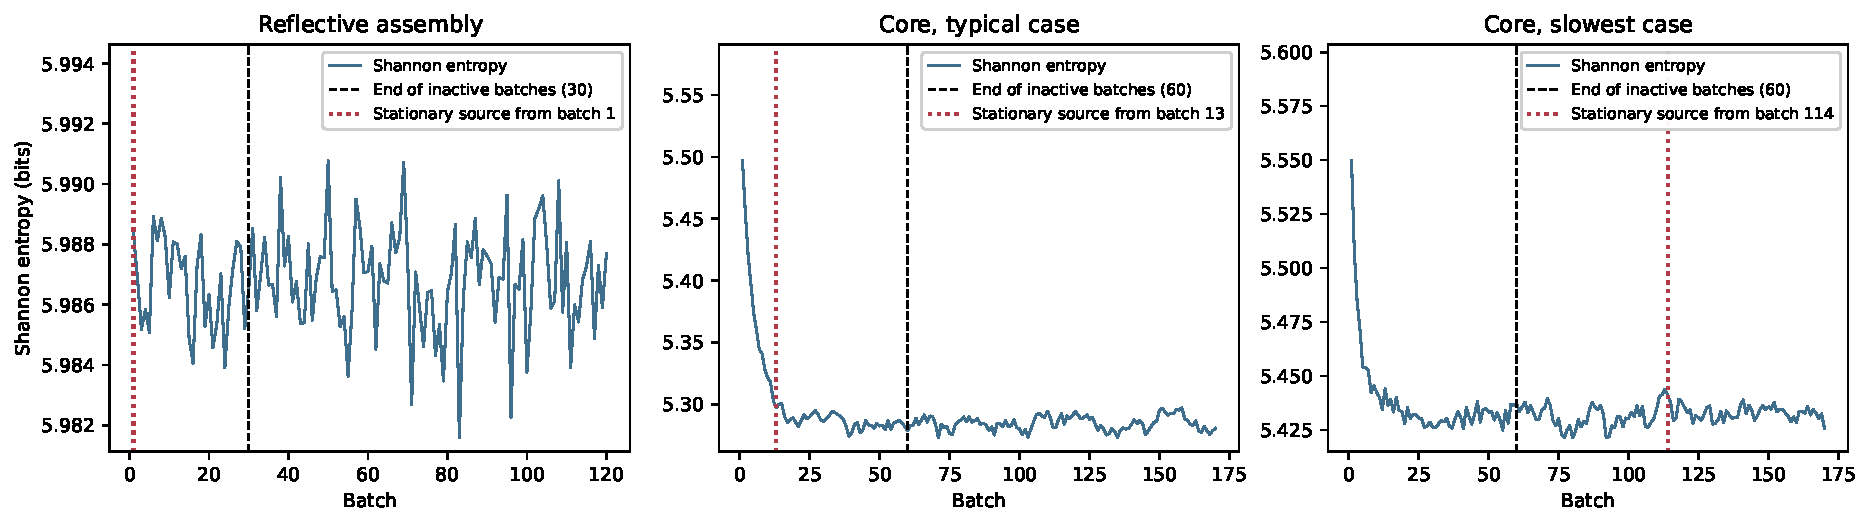
\includegraphics[width=\textwidth]{images/th_entropy.pdf}
          \caption{Shannon entropy per batch: reflective assembly, typical core solve and slowest core solve.}
          \label{fig:entropy}
        \end{figure}

  \item \textbf{Computing environment:} Table~\ref{tab:host-specs}
        gives the processor, memory, operating system and campaigns of
        each host. Both hosts run the same Conda environment, defined in
        the repository, with Python 3.13.13, OpenMC 0.15.3,
        pymoo 0.6.2 and scikit-learn 1.9.0.

\begin{table}[htbp]
  \centering
  \small
  \caption{Computing hosts: configuration and campaigns.}
  \label{tab:host-specs}\label{tab:hosts}
  \begin{tabularx}{\textwidth}{@{}l>{\raggedright\arraybackslash}X>{\raggedright\arraybackslash}X@{}}
    \toprule
    Characteristic & Cloud instance & Workstation \\
    \midrule
    Machine & AWS EC2 c7a.8xlarge, on demand & wks720 \\
    Processor & AMD EPYC 9R14, fourth generation (Genoa) & AMD Ryzen Threadripper 2990WX (Zen+, 12\,nm) \\
    Physical cores & 32 & 32 \\
    Logical processors & 32, simultaneous multithreading disabled & 64, two per core \\
    Clock frequency & Up to \SI{3.7}{GHz} & \SI{3.0}{GHz} base, \SI{4.2}{GHz} boost \\
    Memory & \SI{64}{GiB} & \SI{62}{GiB} available to the operating system \\
    Operating system & Ubuntu Server 24.04, Docker container & Linux Mint 22, kernel 6.8 \\
    Environment & Docker image with the pinned Conda environment & Pinned Conda environment, no administrative privileges \\
    Campaigns & 1, 2, 6 and 7 & 3 to 5, 8 and 9 \\
    \bottomrule
  \end{tabularx}
\end{table}

  \item \textbf{Sources of randomness:} three enter a campaign, and they
        differ in whether they are seeded.

        \begin{enumerate}
          \item Each transport solve is seeded from its own design
                vector (Section~\ref{sec:meth-fidelity}), so every
                archived design reproduces its result.

          \item The Gaussian-process hyperparameter optimisation and
                the NSGA-II search on the surrogate are seeded, so the
                same archive yields the same infill batch.

          \item The Latin-hypercube design of experiments is not
                seeded. The sampling routine of the framework declares a
                seed argument but never forwards it to the pymoo
                Latin-hypercube operator, which is therefore constructed
                without one and samples from the global state of the
                NumPy generator. Three launches with the same configured
                seed returned three different initial design matrices.
                The same routine generates the space-filling designs
                that complete a batch when the sequential selection
                under the minimum-distance constraint
                $\delta_\mathrm{min}$ of the batch-diversity revision
                of Section~\ref{sec:meth-acq} exhausts the candidates,
                so those points are not reproducible either.
        \end{enumerate}

        A campaign relaunched from scratch therefore starts from a
        different design of experiments and follows a different
        trajectory. The record of each campaign is its archived
        checkpoint, which stores every evaluated design with its inputs,
        outputs and the fixed hypervolume reference point, and every
        result of Chapter~\ref{ch:results} is computed from it. The
        checkpoints are held in the public code repository of this
        thesis, described in
        Appendix~\ref{app:code-architecture}. The
        surrogate-search study of Section~\ref{sec:meth-nsga-setting} is
        not affected, because it starts from a fixed archive and uses
        only the seeded search.
\end{itemize}


%% labels of the material reported with the campaign costs in the results, kept so that the
%% cross-references of the other chapters still resolve
\label{sec:meth-cost}

%% labels of the material summarised in the reactor model, kept so that the
%% cross-references of the other chapters still resolve
\label{sec:meth-dep-level}\label{eq:t-solve}\label{eq:t-solve-fit}\label{eq:t-step}\label{eq:bateman-asm}\label{eq:t-step-core}\label{tab:dep-level-cost}\label{tab:dep-3d-cost}

